% Modelo de TCC do Bacharelado em Ciência da Computação da UNIFESP 
% Baseado no Modelo de Documentos Academicos do ABNTex2  

\documentclass[	12pt, Times, openright, twoside, a4paper, english, brazil]{abntex2}


\usepackage{cmap}				
\usepackage{times}
\usepackage[T1]{fontenc}			
\usepackage[utf8]{inputenc}		 
\usepackage{lastpage}			
\usepackage{indentfirst}			 
\usepackage{color}				
\usepackage[table]{xcolor}
\usepackage{graphicx}			
\usepackage[portuguese, ruled, linesnumbered]{algorithm2e} 
\usepackage{amssymb} 
\usepackage{glossaries}
\usepackage{float}
\usepackage{multicol,multirow}
\usepackage{adjustbox}
\usepackage[brazilian,hyperpageref]{backref}	 
\usepackage[alf]{abntex2cite}	
\usepackage{datatool} 
\usepackage[justification=centering]{caption}

\usepackage{lscape,pdflscape}
\usepackage{booktabs}
\usepackage{siunitx} 
%\usepackage{pgfplotstable} 
\usepackage{hyperref}
\hypersetup{colorlinks=False,  linkcolor=black,   filecolor=magenta, urlcolor=cyan }
\urlstyle{same}
\usepackage{listings}
\usepackage{booktabs}
\usepackage{stackengine}%
\usepackage{url}
\makeatletter
\g@addto@macro{\UrlBreaks}{\UrlOrds}
\makeatother

\usepackage{color}
\newcommand{\TODO}[1]{{\textcolor{red}{\textsf{TODO: #1}}}}
\newcommand{\TODOR}[1]{{\textcolor{blue}{\textsf{RESP: #1}}}}
\newcommand{\TEXTO}[1]{{\textcolor{magenta}{#1}}}


\definecolor{dkgreen}{rgb}{0,0.6,0}
\definecolor{gray}{rgb}{0.5,0.5,0.5}
\definecolor{mauve}{rgb}{0.58,0,0.82}
\lstset{
  language=Python,                
  basicstyle=\footnotesize,           
  numbers=left,                   
  numberstyle=\tiny\color{gray},  
  stepnumber=2,                             
  numbersep=5pt,                  
  backgroundcolor=\color{white},    
  showspaces=false,               
  showstringspaces=false,         
  showtabs=false,                 
  frame=single,                   
  rulecolor=\color{black},        
  tabsize=2,                      
  captionpos=b,                   
  breaklines=true,                
  breakatwhitespace=false,        
  title=\lstname,                               
  keywordstyle=\color{blue},          
  commentstyle=\color{dkgreen},       
  stringstyle=\color{mauve},     
}
% --- 
% CONFIGURAÇÕES DE PACOTES

\sisetup{  round-mode = places,  round-precision  = 2}

% ---
% Configurações do pacote backref
% Usado sem a opção hyperpageref de backref
  \renewcommand{\backrefpagesname}{Citado na(s) página(s):~}
%   Texto padrão antes do número das páginas
  \renewcommand{\backref}{}
%   Define os textos da citação
  \renewcommand*{\backrefalt}[4]{
  	\ifcase #1 	Nenhuma citação no texto.  	\or	Citado na página #2.%
  	\else Citado #1 vezes nas páginas #2.  	\fi}%
  % ---

  % numeração de figuras e elas 
  \counterwithout{figure}{section}
  \counterwithout{table}{section}

 \setlength{\parindent}{1.3cm}
 \setlength{\parskip}{\onelineskip}
 
   \makeatletter
  \hypersetup{
       	%pagebackref=true,
  		pdftitle={\@title}, 
  		pdfauthor={\@author},
      	pdfsubject={\imprimirpreambulo},
  	    pdfcreator={LaTeX with abnTeX2},
  		pdfkeywords={abnt}{latex}{abntex}{abntex2}{trabalho acadêmico},  colorlinks=false, linkcolor=blue, citecolor=blue,filecolor=magenta,  urlcolor=blue,
  		bookmarksdepth=4}

  \makeatother


  \makeindex



  \titulo{ANÁLISE DE DEMANDA DO RESTAURANTE UNIVERSITÁRIO DO ICT UNIFESP VIA REDES NEURAIS}
  \autor{Douglas Diniz Landim}
  \local{São José dos Campos, SP}
  \data{Outubro de 2020}
  \orientador{Prof. Dr. Marcos Gon\c{c}alves Quiles}
  \instituicao{Universidade Federal de São Paulo -- UNIFESP
    \par
    Instituto de Ciência de Tecnologia
    \par
    Bacharelado em Ciência da Computação}
  \tipotrabalho{Trabalho de Graduação}
  \preambulo{Trabalho de conclusão de curso apresentado ao Instituto de Ciência e Tecnologia – UNIFESP, como parte das atividades para obtenção do título de Bacharel em Ciência da Computação.}

\begin{document}
 
 \frenchspacing 

  % ----------------------------------------------------------
  % ELEMENTOS PRÉ-TEXTUAIS

  % \pretextual

    
  % ----------------------------------------------------------
  % Capa

    \begin{capa}
      \begin{center}
       
\includegraphics[width=.25\textwidth]{logo-unifesp.pdf}
        \vspace*{\fill}
        
        {\ABNTEXchapterfont\large\imprimirautor}
        \vspace*{\fill}
        
        {\ABNTEXchapterfont\bfseries\Large\imprimirtitulo}
        \vspace*{\fill}\vspace*{\fill}
        
       \imprimirlocal
       \end{center}
    \end{capa}


  % Folha de rosto
    \imprimirfolhaderosto*


  % Inserir folha de aprovação
    % \includepdf{folhadeaprovacao_final.pdf}
  %
    \begin{folhadeaprovacao}
      \begin{center}
        {\ABNTEXchapterfont\large\imprimirautor}

        \vspace*{\fill}\vspace*{\fill}
        {\ABNTEXchapterfont\bfseries\Large\imprimirtitulo}
        \vspace*{\fill}
        
        \hspace{.45\textwidth}
        \begin{minipage}{.5\textwidth}
            \imprimirpreambulo
        \end{minipage}%
        \vspace*{\fill}
       \end{center}
        
       Trabalho para apresentar em Outubro/2020:

       \assinatura{\textbf{\imprimirorientador} \\ Orientador} 
       \assinatura{\textbf{Professora} \\ Dra. Daniela Leal Musa}
       \assinatura{\textbf{Professora} \\ Dra. Regina Célia Coelho}

          
       \begin{center}
        \vspace*{0.5cm}
        {\large\imprimirlocal}
        \par
        {\large\imprimirdata}
        \vspace*{1cm}
      \end{center}
      
    \end{folhadeaprovacao}



  % ----------------------------------------------------------

  % Dedicatória

    \begin{dedicatoria}
       \vspace*{\fill}
       \centering
       \noindent
       \textit{ Este trabalho é dedicado aos meus pais que apoiaram e sacrificaram esforços para me manter ativo nessa jornada, a todos os professores que me somaram conhecimentos, oportunidades e esperanças indo além de suas rotinas e agendas em prol do ensino, e principalmente à todos que me motivaram me oferecendo desafios para que eu pudesse enfrentá-los superando meus próprios limites } \vspace*{\fill}
    \end{dedicatoria}

  % Agradecimentos

    \begin{agradecimentos}
        \paragraph{Minha Jornada}
            Minha jornada pela graduação foi marcada por muita persistência, dificuldades e fracassos. Agradeço primeiramente a Deus por me dar fé e alimentar minha persistência e esperança. Apesar de todo o conteúdo técnico das mais de 40 disciplinas do meu curso, o que mais me agregou aprendizado foi o ambiente desafiador desta universidade; que somado à muitas dificuldades pessoais, acidentes, contra-tempos de saúde, profissão e família; constituiu o conjunto perfeito de desafios que me transformou em uma pessoa forte e destemida para enfrentar as cobranças do mercado, mais convicto e perseverante a cada nova tentativa de conquistar meus objetivos. Agradeço à minha família por sempre me apoiar dando tudo de si, aos meus professores que me orientaram e me motivaram, nas reuniões e chats online até nos finais de semana, aos meus amigos universitários, e a todos os colegas e colaboradores que conheci durante a graduação na Unifesp.
            
            \paragraph{Em especial, agradeço:}
                
            À professora Daniela Musa por ser minha primeira coordenadora de curso e orientadora quando ingressei na Unifesp.
            
            Aos professores das disciplinas que formaram minha base de conhecimento da ciência da computação e que me deram grande preparo para as minhas atividades acadêmicas, profissionais e nos diversos processos seletivos que participei no mercado. Aos professores Reginaldo Kuroshu, Bruno Kimura, Àlvaro Fazenda, Regina Coelho, Arlindo Flavio, Antonio Chaves, Ana Luiza e Otavio Lemos.
            
            À professora Camila Bertini  que na disciplina de simulação de sistemas me motivou nos primeiros estudos no tema deste trabalho, com uma realização de correlação com reamostragem de consumo x temperatura em 2016.
            
            À professora Flavia Martins de estatística, que me orientou algumas vezes em sua sala sobre a introdução teórica de predições com redes neurais, sua tese de doutorado foi bem complementar e enriquecedora na fundamentação teórica deste trabalho.
            
            Aos professores Vinícius Veloso e Fabio Faria, por me apresentarem a disciplina de inteligencia artificial. E ao Vinícius Veloso por me orientar na primeira parte deste trabalho e em todo o desenvolvimento de fundamentação teórica da primeira parte.
            
            Ao professor Marcos Quiles por me orientar nesta segunda parte do trabalho, me apresentando desde o início o trabalho com python, tensorflow, scikit learning, sobre as orientações mais específicas do aprendizado da rede neural. Em me orientar nas métricas de avaliação dos modelos e sobre a toda a metodologia experimental, além das revisões no texto final.
            
            À equipe de Data Science e Machine Learning Engineering da empresa 2RP-NET, especialista em análise de fraudes, dados, e trabalhos com aprendizado de máquina em Big-data, da qual recentemente fui integrado em setembro/2020 graças ao aprendizado adquirido neste trabalho acadêmico. E por ter disponibilizado um período extenso da reunião de equipe durante o nosso expediente para discutirmos os resultados e métricas deste trabalho, equipe da qual é composta por profissionais mestres e doutores em data science e machine learning.
            
            À todos os outros professores, colegas, alunos e colaboradores do instituto de ciência e tecnologia da UNIFESP.
                
            À minha família por ter me apoiado nesse longo período na UNIFESP.

         \end{agradecimentos}
 
 
 
  % Epígrafe
  
    \begin{epigrafe}
        \vspace*{\fill}
    	\begin{flushright}
    		\textit{Mesmo desacreditado e ignorado por todos, não posso desistir, pois para mim, vencer é nunca desistir.\\
    		(Albert Einstein)}
    	\end{flushright}
    \end{epigrafe}
 
 
  % ----------------------------------------------------------
  % RESUMOS
 
  % resumo em português
    \begin{resumo}
         O presente trabalho tem como objetivo o estudo de métodos para a previsão de vendas do restaurante universitário da Unifesp para evitar super-projeção de demanda com consequência de desperdício de alimentos, ou subprojeção com consequência de docentes ou discentes sem refeições. Em uma investigação anterior, realizada como trabalho de disciplina, o autor empregou métodos estatísticos para a análise do comportamento de consumo de refeições. Neste trabalho, foram desenvolvidos modelos de aprendizado de máquina, mais especificamente, redes neurais perceptron de múltiplas camadas e redes \textit{gated recurrent units}, com métodos de análises de dados coletados, preparação e pré-processamento das informações, seleção e avaliação dos melhores modelos e conclusões finais.
     
     \vspace{\onelineskip}
        
     \noindent
     \textbf{Palavras-chave}: Redes Neurais Artificiais, Previsão de demanda, Aprendizado de Máquina, Inteligência Artificial, Perceptron Múltiplas camadas. 
     
    \end{resumo}

  % resumo em inglês
    \begin{resumo}[Abstract]
     \begin{otherlanguage*}{english}

% TRADUZIR NOVAMENTE DO RESUMO ALTERADO

        This current work aims to study methods for forecasting meals of Unifesp university restaurant to avoid over-projection of demand resulting from food waste, or under projection with the consequence of teachers or students without meals. In a previous investigation, carried out as discipline work, the author used statistical methods to analyze meal consumption behavior. Machine learning models were developed in this work, more specifically, multilayer perceptron neural networks and gated recurrent units networks, with data analysis methods, preparation and pre-processing of information, selection, and evaluation of the best models and final conclusions.

       \vspace{\onelineskip}
     
       \noindent 
       \textbf{Keywords}: Artificial Neural Networks, Demand Prediction, Machine Learning, Artificial intelligence, Perceptron Multiple layers.
     \end{otherlanguage*}
    \end{resumo}


  % ----------------------------------------------------------
  
  % Lista de ilustrações
    \pdfbookmark[0]{\listfigurename}{lof}
    \listoffigures*
    \cleardoublepage

  % Lista de tabelas
    \pdfbookmark[0]{\listtablename}{lot}
    \listoftables*
    \cleardoublepage


  % ---  % Lsta de abreviaturas e siglas
  % ---
    \begin{siglas}
    \item[ICT] Instituto de Ciência e Tecnologia
    \item[R.U.] Restaurante Universitário
    \item[UNIFESP] Universidade Federal de São Paulo
    \item[UFV] Universidade Federal de Viçosa
    \item[UNESP] Universidade Estadual Paulista Júlio de Mesquita Filho
    \item[BDMEP] Banco de Dados Meteorológicos para Ensino e Pesquisa
    \item[RNA] Rede Neural Artificial
    \item[MLP] Multi Layer Perceptron
    \item[GRU] Gated Recurrent Unit
    \item[RMSE] Root Mean Squared Error

    \end{siglas}
 
  % ---
    \pdfbookmark[0]{\contentsname}{toc}
    \tableofcontents*
    \cleardoublepage
  % ---



  % ----------------------------------------------------------
  % ELEMENTOS TEXTUAIS
  % ----------------------------------------------------------
  \textual

  % ----------------------------------------------------------
  % CAPÍTULO 1 - Introdução
  % ----------------------------------------------------------
  
    \chapter{Introdução}

% \section{Contextualização e Motivação}

\noindent

Dentre as definições mais aceitas sobre segurança alimentar está a versão cunhada durante a Cúpula Mundial da Alimentação de 1996 \cite{shaw2007world}, que a enuncia como uma situação em que todas as pessoas, a todo momento, tenha condições física, social e econômica de acesso a alimentação segura, saudável e nutritiva para uma vida saudável e ativa. Porém, Segundo a Organização Mundial da Saúde \cite{world2009global} mais de 1 bilhão de pessoas no mundo possuem uma dieta nutritivamente insuficiente e mais que o dobro de pessoas tem carência de micronutrientes.

Segundo \citeonline{webb2006} a segurança alimentar pode ser decomposta em 3 pilares essenciais, disponibilidade, possibilidade de acesso e utilização racional. Estes conceitos são intrinsecamente hierárquicos uma vez que a disponibilidade não garante acesso, que por sua vez não garante sua utilização racional. Com os avanços na produção agrícola e a abertura dos mercados econômicos mundiais, ainda que não tenha solucionado o problema, possibilitou passos largos nos dois primeiros pilares da segurança alimentar supracitados. Assim, nas primeiras décadas do século XXI o terceiro pilar, da utilização racional dos recursos, tem se mostrado um importante fator a ser considerado neste novo mundo globalizado \cite{barrett2010}.

No final do ano de 2019 uma doença altamente transmissível foi identificada na província de Wuhan na china, comumente chamada de o novo Coronavírus (COVID-19), a qual foi declarada estar em estado de  pandemia em março de 2020, e até o presente momento infectou mais de 40 milhões de pessoas e ocasionou 1 milhão de mortes\footnote{\url{https://www.worldometers.info/coronavirus/}}. Ainda que com esforços globais para contenção e remediação da pandemia de COVID-19, não existem vacinas ou curas cientificamente comprovadas e a necessidade de \textit{lockdown} ainda é pertinente para evitar novas ondas de contaminação. Os efeitos da pandemia foram devastadores em praticamente todas as áreas econômicas, principalmente o setor de alimentação que é essencial para a manutenção da vida e não tem espaço para \textit{lockdown} \cite{galanakis2020food}.

No dia 22 de julho de 2020, a Associação Brasileira da Indústria e Consumo de alimentos, realizou uma conferência sobre os impactos da pandemia do COVID-19 na cadeia produtiva brasileira de alimentos \footnote{\url{{https://www.abia.org.br/noticias/abia-participa-de-live-para-discutir-os-impactos-da-pandemia-na-cadeia-produtiva-de-alimentos}}}. Nesta conferência foram reunidos especialistas e executivos do setor agroindustrial para analisar mudanças de comportamento de consumo nos setores terciários que lidam diretamente com o fornecimento de alimentos ao consumidor final. A partir desta análise da nova rotina do consumidor, estão sendo buscados novos métodos de se prever o formato atual de consumo e a nova demanda para estes setores. Por fim, foram discutidos também métodos de produção e abastecimento do agronegócio para o setor terciário.

Assim, neste período caótico, em que a mão de obra global reduziu aproximadamente 25\% durante os primeiros meses de pandemia \cite{huff2015resilient}, vem atona a importância do desenvolvimento de processos que utilizem os recursos alimentícios da forma mais racional possível. Neste contexto, uma área que chama a atenção é a de previsão de demandas indústrias ou de estabelecimentos que lidam com alimentos perecíveis em grande quantidade, uma vez que o alimento tem prazo de validade e a produção por demanda pode evitar armazenamento por longos períodos ou descartes indesejado de alimentos prontos para consumo.

Neste sentido, tornam-se viáveis a previsão de demandas para refeições em restaurantes industriais ou de grande porte, como os restaurantes universitários (RU) em que são ofertadas refeições a preços acessíveis para a comunidade estudantil da instituição, através de subsídios no valor repassado aos alunos. Geralmente os RU's são terceirizados por meio de licitações em que o governo do estado uma porcentagem de cada refeição produzida para a empresa gestora do restaurante. Devido a regulamentações sanitárias, refeições preparadas mas não consumidas até o final do expediente devem ser descartadas para evitar contaminações e garantir a segurança alimentar do consumidor \footnote{\url{https://super.abril.com.br/mundo-estranho/o-que-acontece-com-a-comida-que-sobra-dos-restaurantes/}}. Dessa forma, a produção em excedente (não consumida) de refeições por parte dos RU's gera não somente um gasto exagerado de recursos financeiros públicos mas também uma utilização pouco racional dos recursos alimentícios.

Neste contexto, o restaurante universitário da Unifesp em São José dos Campos é um bom estudo de caso uma vez que vende aproximadamente 90 mil refeições anualmente, em que cada refeição tem o valor fixo de R\$2,50 para alunos e um subsidio médio de aproximadamente R\$9,00 por refeição na ultima década (2011-2019). Com isto, foram subsidiados mais de 6 milhões de reais durante os anos de 2011 a 2019.

Uma forma de se reduzir esse desperdício está na desenvolvimento de métodos de predição de consumo \cite{Lopes2008,Rocha2011}. Normalmente, as abordagens para previsão da demanda de consumo de um restaurante universitário se resumem a análise exploratória de dados coletados, como por exemplo, as vendas computadas na semana ou mês anterior. Além disso, informações externa, denominadas dados exógenos, também podem ser considerados no processo de predição, como por exemplo dados climáticos, dados do calendário anual, feriados, dentre outras informações que podem ser relevantes para a estimativa de consumo.

A predição de consumo de redes restaurantes universitários já foi abordada em outros trabalhos. Por exemplo, no trabalho de \citeonline{Lopes2008} realizado na UFV, é utilizado um modelo de rede neural perceptron de 1 camada oculta e 1 neurônio de saída, utilizando os 5 dias anteriores como parâmetros de predição com erro de 3\% sobre o total consumido, e no trabalho de \citeonline{Rocha2011} realizado na UNESP é utilizado também um modelo de rede neural com 1 camada oculta e 1 neurônio de saída, utilizando apenas 1 parâmetro que informa o número de refeições do dia anterior, e outros parâmetros informando médias de dias anteriores e informações relativas à data de consumo, este modelo obteve erro de 9,5\% calculado sobre o total consumido.

Assim, este trabalho consiste na aplicação de modelos de redes neurais para a previsão de demanda das refeições fornecidas no restaurante universitário da Unifesp no campus de São José dos Campos. Para isso, será utilizado um conjunto de dados históricos disponíveis no sistema da Unifesp e outras informações externas (exógenas) que podem impactar o comportamento de consumo e seu processo de predição.

Os objetivos gerais deste trabalho compõem a construção e comparação de modelos de Redes Neurais Artificiais para a previsão da demanda de refeições do restaurante universitário do ICT-UNIFESP. Especificamente, tem-se como objetivos:
\begin{enumerate}[label=\alph*)]
\item Obter e preprocessar os dados de consumo e venda de refeições do ambiente do restaurante e dados do ambiente externo ao consumo, como por exemplo dados climáticos, visando seu uso como entrada de modelos de aprendizado de máquina para a obtenção das predições de consumo na saída destes modelos;
\item Realizar análises exploratórias e descritivas de todos os dados;
\item Construir e avaliar modelos preditivos de redes neurais;
\item Realizar análises sobre as métricas de predições dos modelos apontando suas características viáveis para uma predição de consumo.
\end{enumerate}

O restante deste documento está organizado da seguinte forma. O capítulo \ref{cap:teoria} introduz a fundamentação necessária a compreensão deste trabalho; A literatura relacionada ao tema é descrita no capítulo \ref{cap:literatura}; O capítulo \ref{cap:metodos} apresenta a metodologia empregada nesse estudo; Os resultados são sumarizados no capítulo \ref{cap:resultados}; As principais conclusões desse trabalho bem como as indicações de investigações futuras são apresentadas no capítulo. \ref{cap:conclusoes}; Por fim, o capítulo \ref{cap:anexo1} apresenta alguns resultados adicionais gerados durante os experimentos e os códigos implementados.

    \chapter{Fundamentação teórica} \label{cap:teoria}
  
Neste capítulo será feita uma breve revisão das características principais das series temporais,  assim como das redes neurais, especialmente das que serão aplicadas no problema de interesse, chamadas de redes Multilayer Perceptron (MLP) e redes Gated Recurrent Unit (GRU).  

    \section{Métodos de Previsão de Demanda} 
    
        A previsão de demanda pode ser definida como um processo de busca de informações que geram vendas de um produto ou um conjunto de produtos.
        
        Em \citeonline{moreira1998} são definidos os métodos de previsão de demanda como processos que utilizam tais informações para estimar uma demanda futura, podendo se encaixar nesta definição desde métodos subjetivos e intuitivos até métodos matemáticos e computacionais. No mesmo trabalho, são classificado os modelos de previsão em dois grandes grupos: métodos qualitativos e métodos quantitativos.
        
         Em  \citeonline{Junior2007} foi feito a avaliação de  diversos métodos de previsão de demanda, os quais são esquematizados na Figura \ref{fig: metodosPrevisaoDemanda}. 
        
                  \begin{figure}[ht]
                  	\center{
                  	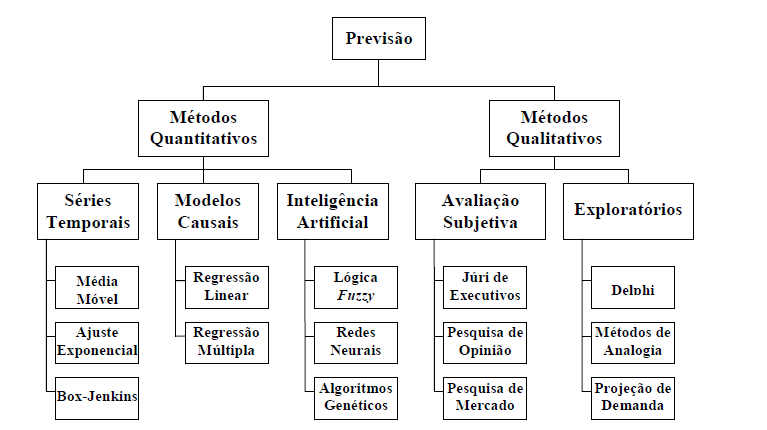
\includegraphics[width=\textwidth]{./Figs/01-junior-metodos-previsao-demanda.png}
                  	\caption{Métodos de previsão de demanda.}\caption*{  Fonte: \cite{Junior2007}.}
                  	\label{fig: metodosPrevisaoDemanda}}
                  \end{figure}
        
        Os métodos qualitativos são definidos em \cite{Junior2007} como um julgamento dos dados expostos sem processamento analítico, tais como agrupamento e classificação de dados. Esses métodos não fornecem novas informações numéricas nem  modelos preditivos.
        
        Já os métodos quantitativos são definidos, no mesmo trabalho, como sendo analíticos e baseados em  modelos matemáticos para realizar previsões. Esses métodos analisam padrões de comportamento de um histórico de dados, visando predizer comportamento futuro.
         
        Em \citeonline{Junior2007} também é mencionado que os dados coletados para modelos de previsão, ao ser projetados graficamente, evidenciam comportamentos que podem ser generalizados de forma subjetiva pelos gestores dos dados. Em todos os casos, a análise de dados é necessária para selecionar parâmetros de demanda objetivos para fazer predições. Porém, apenas a análise dos dados pode ser insuficiente,  e se realizada com critérios incorretos pode comprometer as conclusões dos estudos. 
        
        A análise de dados é um processo amplo que visa tratar os dados desde sua aquisição e pré-processamento até a sua interpretação a partir de ferramentas complexas de mineração. Nas diferentes etapas, são abrangidas diversas técnicas matemáticas, probabilísticas, estatísticas, computacionais e heurísticas.  Na Seção \ref{sec: timeseries} serão comentadas as principais características das séries temporais, o qual será o método de previsão aplicado ao problema prático de interesse. 
    
        \subsection{Séries Temporais} \label{sec: timeseries} 
         
            De acordo com  \citeonline{Morettin1987}, uma série temporal é um conjunto de observações ordenadas em função do tempo, comumente iguais, apresentando uma dependência serial entre ela. Também pode ser definida como uma realização de um conjunto de variáveis aleatórias $ X=\{x_1, x_2, \dots, x_T\}$, ordenadas no tempo, onde  $T$ representa o comprimento da série, como é feito em \cite{defts}. A relação entre as variáveis é comumente descrita pela função de distribuição conjunta delas, ou, em outros casos, pela media e covarianças. 
            
            Entre os objetivos do análise de séries temporais, podem ser destacados os seguintes: i) descrever o comportamento das séries identificando tendências e variações, ii) analisar e modelar  a dependência entre as observações, e iii) fazer previsões de valores futuros da série. 
            
            As series temporais tem uma componente determinística e uma componente aleatória, e podem ser contínuas ou discretas, dependendo do tipo de observação das variáveis. São chamadas de estacionárias quando as propriedades de média, variança e covariança são mantidas no tempo. A tendência faz referência à taxa de crescimento ou de decréscimo, podendo ser linear, exponencial ou amortecido. Já a oscilação da tendência é conhecida como ciclo. Além disso, podem apresentar sazonalidade, isto é, exibir comportamento que tende a se repetir em certo numero de períodos de tempo.
    
            Exemplos de cada uma dessas propriedades, assim como técnicas aplicadas para estudo e correção de cada uma delas podem ser vistas em \cite{tecnicas1}. Essas características, junto com o estudo da componente aleatória, fornecem informações de interesse para as aplicações práticas.  
            %\TODOR{Passar pra metodologia ou literatura, não falar do trabalho aqui}
            Devido ao objetivo deste trabalho, serão aplicadas series temporais para eventos com sazonalidade, a fim de estimar previsões. As técnicas para fazer isto usam métodos de regressão,  e algumas aplicações praticas podem ser vistas incluem  previsão de consumo de energia elétrica realizados , como feito em  \citeonline{Almeida2013}, \citeonline{RUAS2012} e \citeonline{Silva2010}, e da previsão de demanda de produtos cosméticos, como pode ser visto em \citeonline{Junior2007}.
    
    \section{Redes Neurais Artificiais}
    
        As redes neurais artificiais são ferramentas com raiz multidisciplinar, pois são nutridas por conhecimentos de neurociência, matemática, estatística, física, ciência da computação e engenharia \cite{Haykin1994}, e fazem parte da grande área de conhecimento denominada Inteligência Artificial (IA), termo cunhado em \cite{kaplan2019siri}.
        
        De forma resumida, poderia ser definido que "a inteligência artificial é o ramo da ciência da computação que se ocupa do comportamento inteligente." \cite{Luger2004}. Os sistemas de inteligência artificial buscam resolver funções e problemas inspirados em duas características humanas: capacidade de abstração e aprendizagem com o erro. 
        
        No contexto de IA um neurônio é uma unidade considerada fundamental para o processamento de informação, e as redes neurais são conjuntos de neurônios artificiais interconectados através de relações, funções lógicas e matemáticas \cite{Haykin1994}. Os neurônios de uma rede são capazes de processar múltiplos valores de entradas e reagir rapidamente produzindo uma resposta relacionada à essas entradas, simulando o comportamento do cérebro humano. 
        
        Inspirado por uma busca de um modelo computacional do neurônio biológico, o primeiro modelo de neurônio artificial, denominado MCP, foi proposto no artigo \textit{ A Logical Calculus of the Ideas Immanent in Nervous Activity.} \cite{mcculloch43a}, uma ilustração adaptada por \cite{lemos} deste modelo pode ser visualizada na figura \ref{fig: NeuronioArtificial}.
        
        McCuloch era psiquiatra e neuroanatomista e passou cerca de 20 anos refletindo e estudando sobre a representação do sistema nervoso, em 1942 ele convidou Pitts, que era matemático, para fazer parte das suas pesquisas.
        
        A estrutura do neurônio artificial reage a um vetor de entradas e as sinapses são representas por pesos numéricos. Uma função de transferência, também chamada função de ativação, avalia uma combinação linear dos valores da entrada e os pesos das sinapses, determinando se o neurônio é ativado ou não dependendo do valor obtido. Se o neurônio é ativado é emitido um valor de saída 1, caso contrário se emite um valor de saída 0.
            \begin{figure}[ht]
                \center{
                  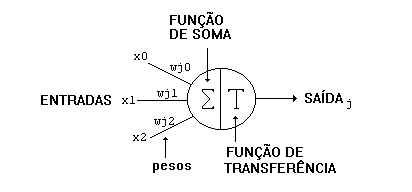
\includegraphics[width=0.65\textwidth]
                  {./Figs/02-neuronio-artificial.png}
                \caption{Neuronio Artificial. }\caption*{  Fonte:\cite{lemos}} \label{fig: NeuronioArtificial} }
            \end{figure}
            
        Todo o funcionamento deste modelo então é reduzido a responder se a soma ponderada recebida é maior que um valor numérico estabelecido. Contudo, associado a este neurônio não foi proposto uma forma automática para ajuste dos pesos, ou seja, não foi dado um algoritmo de aprendizagem para treinar o neurônio. Esse problema foi contornado posteriormente, pela formulação do Perceptron.
        
        Em \citeonline{Haykin1994} no capítulo 1.9 denominado \textit{Notas Históricas}, é apresentada com mais detalhes a fascinante história de desenvolvimento das redes neurais desde a concepção inicial do estudos do neurônio biológico até redes complexas de aprendizagem supervisionada chamadas de \textit{Máquinas de Vetor Suporte}.
            
        \subsection{Perceptron} \label{sec: perceptron}
    
            O modelo de neurônio proposto em \citeonline{mcculloch43a}, apesar de simular um neurônio biológico e resolver algumas tarefas lógicas e matemáticas, não atendia o objetivo principal da Inteligência Artificial: A capacidade de aprendizado. Para poder utilizar esta estrutura, era necessário conhecer o ajuste dos pesos das entradas, o qual não era um problema trivial em muitos casos. 
                        
            O primeiro neurônio com um algoritmo de aprendizado foi proposto em \citeonline{perceptron} e foi nomeado de Perceptron. Nesse trabalho, os pesos das conexões são ajustados de forma autônoma com a introdução de pesos associados e um valor bias, a fim de buscar um reconhecimento autônomo de padrões. Na Figura \ref{fig: perceptron} é apresentado um esquema do funcionamento da estrutura.
            
            \begin{figure}[ht]
            	\center{
              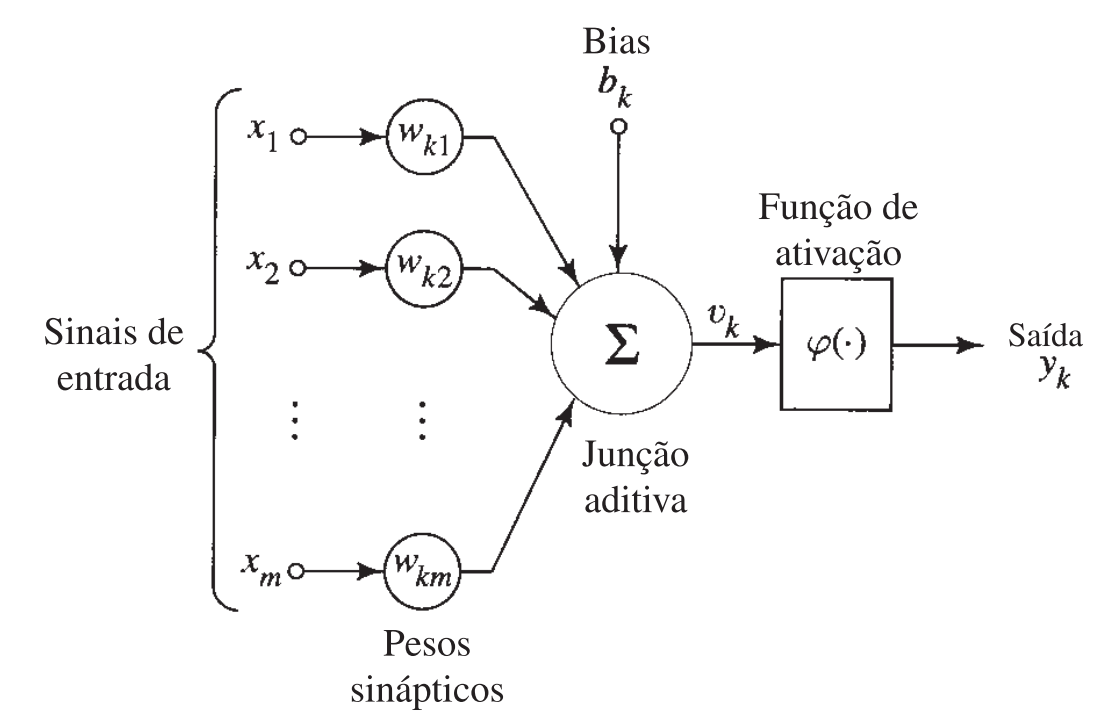
\includegraphics[width=0.65\textwidth]
              {./Figs/03-perceptron.png}
            \caption{Neurônio Artificial Perceptron. }\caption*{  Fonte: \citeonline{Haykin1994}} \label{fig: perceptron} }
            \end{figure}
            
            Porém, em \citeonline{perceptrons2} foi provado que, devido ao modelo aprendizado limitado a uma combinação linear, o perceptron poderia resolver apenas problemas linearmente separáveis. Na Figura \ref{fig:problemasLineares} são apresentados dois problemas simples, um que o perceptron pode resolver \textit{(a)}, e outro que não \textit{(b)}.
            
            \begin{figure}[ht]
              	\center{
              	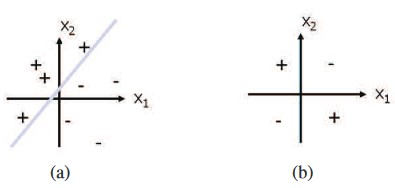
\includegraphics[width=0.8\textwidth]{./Figs/04-limite-perceptron.jpg}
              	\caption{Problema linearmente separável (a) e não separável (b).}\caption*{  Fonte:\cite{Flavia2014}.}
              	\label{fig:problemasLineares}
              	}	
            \end{figure}
            
            Quase duas décadas depois, foi apresentado em \cite{rede1} o primeiro modelo de rede neural, chamada de rede perceptron, aplicando o treinamento por combinações lineares à um conjunto de perceptrons interligados. Essa abordagem permitia resolver problemas mais complexos por meio de uma combinação de soluções. 
              
            A rede possuía apenas uma camada de entrada, uma única saída, e uma função de ativação  $ \varphi $ \cite{Haykin1994}. A função de ativação da rede perceptron ainda poderia ser linear ou não linear. Na Figura \ref{fig:activation_functions} são ilustradas algumas funções de ativação comumente utilizadas. 
            
             \begin{figure}[ht]
                \center{
            	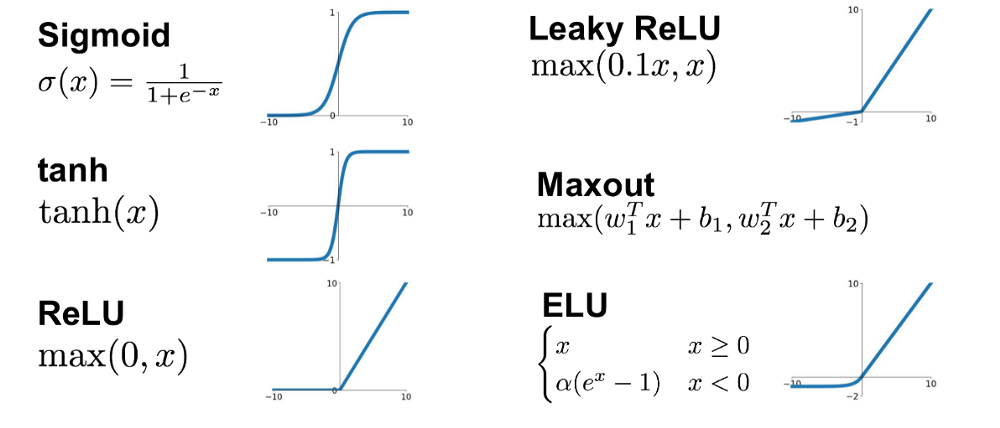
\includegraphics[width=0.80\textwidth] {./Figs/05-funcoes-ativacao.png}
                \caption{Exemplos de funções de Ativação.}\caption*{  Fonte: \cite{MCAI}} \label{fig:activation_functions}} 
            \end{figure}
            
            Em \citeonline{Almeida2013} é analisado o processo de aprendizado da rede perceptron, de forma supervisionada. Neste processo, a estrutura aprende a relacionar um conjunto observado de variáveis de entrada na rede com um ou mais valores de saída esperados denominado como valores reais ou valores verdades. Depois são avaliados os resultados do aprendizado, comparando estes valores com os valores gerados pela rede perceptron sobre o mesmo conjunto de dados, e partir desta comparação é calculada a medida de erro do treinamento.
                        
            Um critério de parada do algoritmo de treino é verificar se o erro é aceitável ou não. Caso afirmativo, a rede neural mantêm os valores dos pesos das sinapses obtidos no momento. Caso contrário, é feita uma nova época de treino tentando ajustar os pesos para obter um erro menor.
            O outro critério de parada é atingir um numero máximo permitido de épocas de treinamento. O reajuste de pesos é denominado taxa de aprendizagem.
            
            O seguinte passo no desenvolvimento de modelos de redes neurais está relacionado com a topologia que determina a quantia dos perceptrons na rede e a forma como eles se conectam, gerando redes de múltiplas camadas.        
    
        \subsection{Rede MultiLayer Perceptron (MLP)}
    
            A possibilidade de combinar duas ou mais camadas de perceptrons foi dada pela utilização de um perceptron combinador de sinal de saída. Com ele as redes neurais são ampliadas para varias colunas de perceptrons interconectados. Cada coluna é denominada uma camada oculta da rede neural. A ultima camada deve ter o número de perceptrons correspondente ao número de saídas desejadas. Na Figura \ref{fig:MLP} é apresentada  uma rede neural com 2 camadas ocultas, e cuja camada de saída possui 3 neurônios.
            
            \begin{figure}[ht]
             \center{
             	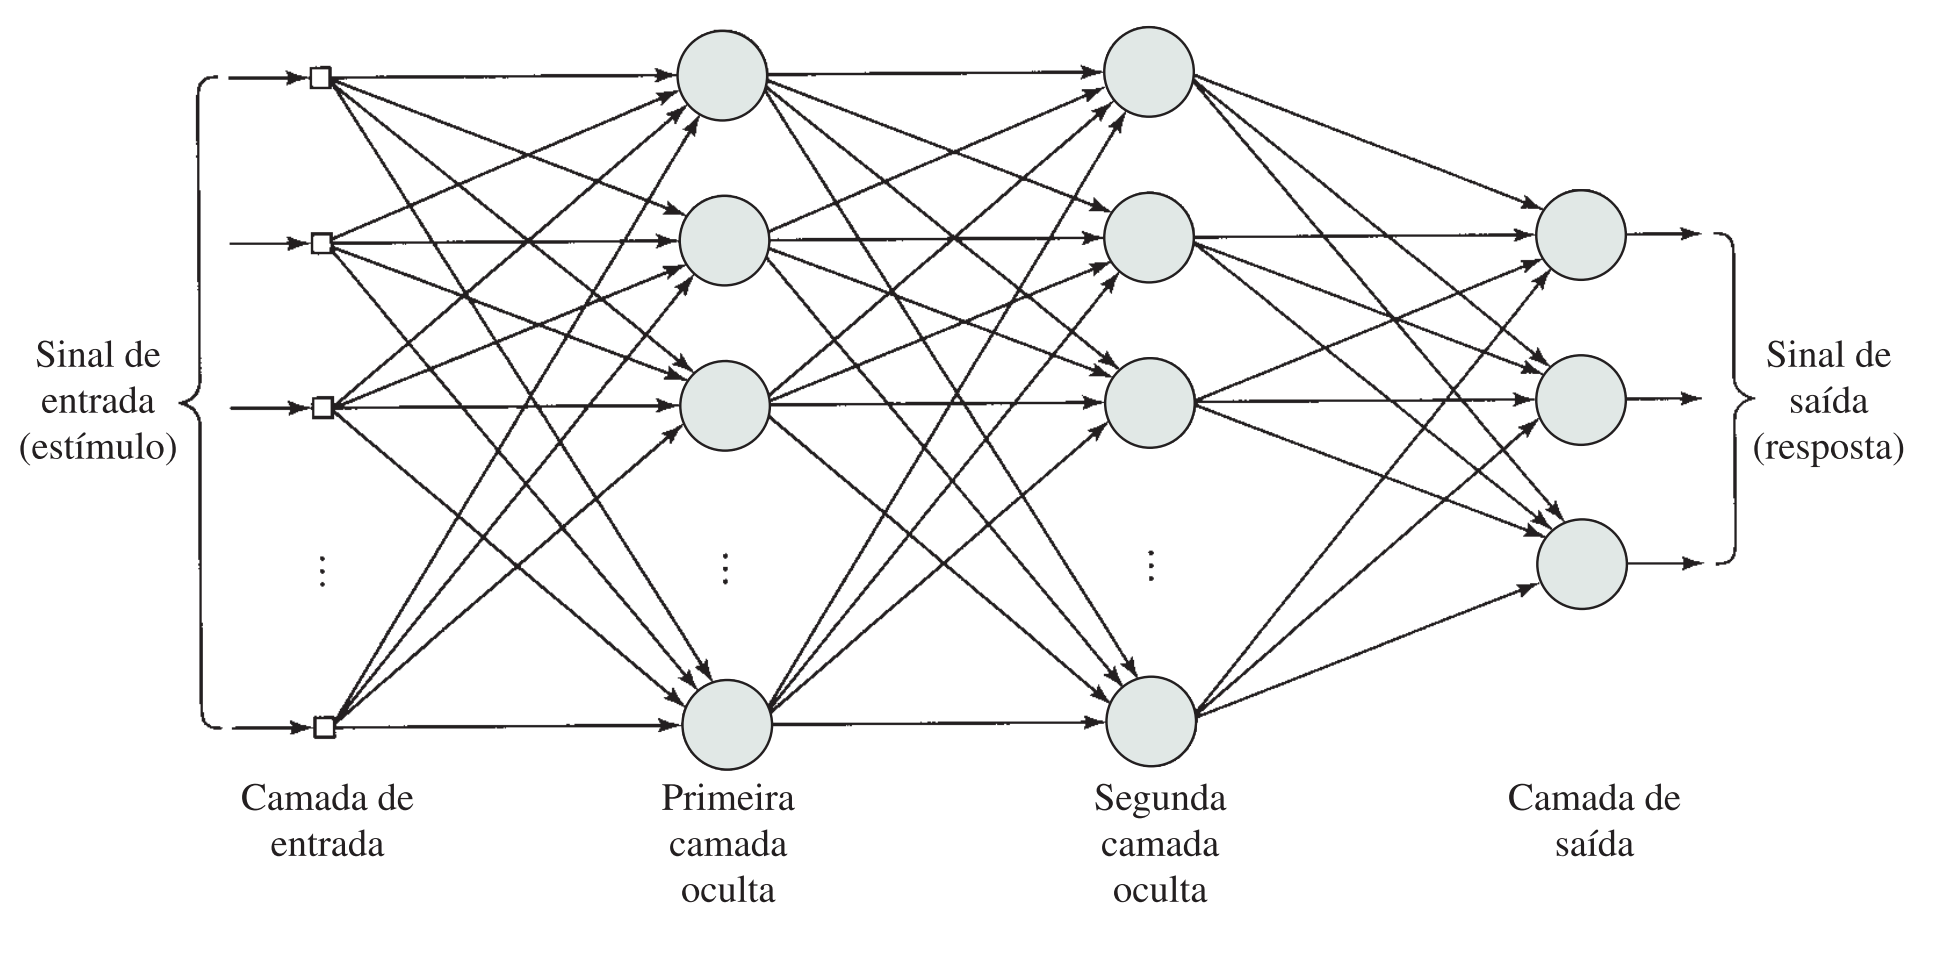
\includegraphics[width=\textwidth]
             	{./Figs/06-MLP.PNG}
             \caption{Rede de perceptrons com múltiplas camadas. }\caption*{  Fonte: \cite{Haykin1994}\label{fig:MLP}
             }}
            \end{figure}
            
            Em \citeonline{Braga2000} é postulado que através de uma camada intermediária é possível aproximar qualquer função contínua e, ainda mais, que duas camadas intermediárias são suficientes para aproximar qualquer função matemática. Se a utilização de duas ou mais camadas pode facilitar o treinamento da rede, torna-se inviável a utilização de um número grande destas, pois em cada camada oculta o erro é estimado a partir do erro na camada anterior, o que gera perda de precisão.
            
            Nas aplicações práticas, tem-se visto que em alguns casos, que a capacidade de abstração e reconhecimento de padrões das redes neurais sobrepassa as capacidades humanas. Em outros casos, uma rede pode não produzir uma resposta esperada resolvendo erroneamente um problema, assim como o cérebro humano, devido à limitações de aprendizado ou falhas nos treinos. 
              
            Para treinar de modo supervisionado uma rede MLP, o conjunto de dados de entrada deve ser dividido em em dois subconjuntos, um de \textit{treino} e um de \textit{validação}. Esses subconjuntos podem ser separados com diversas técnicas. Assim, por exemplo em \citeonline{DLB} é apresentada uma forma heurística de separação de conjuntos em ordem aleatória, com 70\% dos dados para treino e 30\% dos dados para validação.
            
            Em relação ao numero máximo de tentativas de treino permitidas, tem-se que treinos muito prolongados tendem a memorizar pesos dos valores observados nos dados de treino. Isto se traduz em perda capacidade de generalização da rede, implicando em uma dificuldade para avaliar entradas fora dos dados de treino. Esse fenômeno é conhecido como \textit{overfitting}.
            
            Existe uma outra forma de treinar uma rede MLP, chamada de validação cruzada, que foi apresentada em \cite{crossvalidation}. Essa técnica consiste em intercambiar os conjuntos de treino e de validação em diferentes épocas de treino. Nesse caso, a medida do erro de validação passa por um processo de avaliação levando em consideração o número de épocas. Avaliando o erro quadrático médio de ambos os conjuntos é possível detectar o inicio do \textit{overfitting}. Por isso, o ponto ótimo de parada do treinamento está associado ao limite inferior deste erro quadrático médio no conjunto de validação ilustrado na figura \ref{fig:validacaoCruzada} como ponto de parada antecipada ao \textit{overfitting}.
            
            \begin{figure}[ht]
              \center{
              	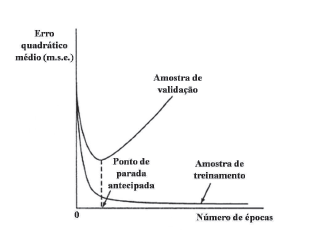
\includegraphics[width=0.5\textwidth]
              	{./Figs/07-validacaocruzada.png}
              
              \caption{Ponto ótimo de parada da validação cruzada. }\caption*{ Fonte: \cite{Haykin1994}} \label{fig:validacaoCruzada}} 
            \end{figure}
    
        \subsection{Rede perceptron Múltiplas Camadas com \textit{Backpropagation}.}
    
            O método de aprendizado para redes neurais de múltiplas camadas denominado de \textit{Backpropagation} foi apresentado em \cite{backp}, como abreviação de \textit{backward propagation of errors}, em português, retro-propagação de erros. Nesse método, o treinamento é feito em duas fases:
        
            \paragraph*{\textit{ Feed-forward} } E apresentado um vetor de entrada com vetor de saída conhecido aos neurônios da primeira camada, e calculado um vetor de saída seguindo o fluxo natural das operações na rede.
             
            \paragraph*{\textit{Feed-backward}} É calculado o gradiente do erro, para obter informação que induz decréscimo na função, dada pela direção oposta ao gradiente. Com isso, são atualizados os pesos de todas as camadas, começando pela última e seguindo o fluxo inverso da rede.
             
            Essas duas fases são esquematizadas na Figura \ref{fig: MLP2}. 
             
            \begin{figure}[ht]
             	\center{
             		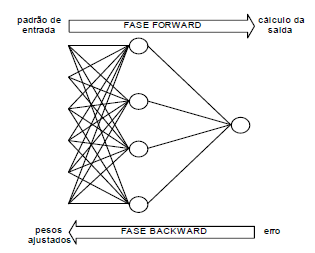
\includegraphics[width=0.65\textwidth]
             		{./Figs/08-mlp-back.png}
             	
             	\caption{Fases de treino da \textit{MLP-Back-Propagation}.}\caption*{  Fonte:  \cite{Almeida2013}}\label{fig: MLP2}}
            \end{figure}
            
            Neste método, a medida que o gradiente do erro é calculado das camadas inferiores para as superiores, sua norma  decresce com velocidade exponencial. Isto faz que nas camadas mais próximas à entrada os ajustes de pesos  sejam pequenos, tornando o aprendizado nelas  mais lento. Este problema é conhecido na literatura como \textit{vanishing gradient problem}, o problema de dissipação do gradiente.   Usualmente, os valores das taxas de aprendizagem ficam entre 0,2 e 0,8.
            
            Nos treinamentos de redes neurais MLP com \textit{backpropagation}, a validação ocorre só com a fase \textit{feedforward}, obtendo-se os erros quadráticos da camada de saída com o dado de validação observado. 
            
            Como o ponto ótimo de parada é um limite inferior, o mesmo somente é descoberto quando superado após algumas épocas de treino, dado que em procedimentos práticos a obtenção de erro é oscilatória e pelo qual é necessário manter salvos os parâmetros obtidos durante estas épocas.
            
            \paragraph{Otimizador de reajuste dos pesos} São conhecidos vários algoritmos que otimizam a convergência do reajuste dos pesos no treino de \textit{backpropagation}, como os que serão mencionados a seguir. O otimizador Momentum acelera o reajuste dos pesos em busca dos erros globais mínimos, e o RMSProp impede a busca na direção das oscilações. Um terceiro otimizador, denominado Adam pela abreviação de Adaptive Moment otimization, combina essas duas caracterpisticas. Para o algoritmo ADAM, a taxa de aprendizado pode ser arbitrada mas em \citeonline{MLM} é mencionado que uma constante com valor 0.001 tem produzido resultados positivos em problemas de predições.  
            
            Na Figura \ref{fig:otimizadores} é comparado  o comportamento de alguns otimizadores. Nesta figura é possível ver que quanto menor o custo de treinamento, maior a velocidade de convergência ao reajuste ideal dos pesos. Além disso, é visível a vantagem computacional do ADAM frente à outros otimizadores, quando se aumenta o número de iterações.
            
            \begin{figure}[ht]
            \center{
            	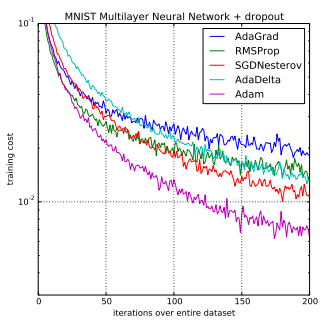
\includegraphics[width=0.70\textwidth]
            	{./Figuras/MLM/optimizers.png}
            
            \caption{Comportamento de otimizadores para MLP treinadas com \textit{Backpropagation}.}\caption*{  Fonte : \cite{MLM} }    \label{fig:otimizadores}}
        
            \end{figure}
            
    \subsection{Redes Recorrentes: O modelo GRU}\label{sec:GRU}

    As redes GRU, abreviação de \textit{Gated Recurrent Unit}, foram apresentadaspor primeira vez em \cite{gru}, sendo uma adaptação das redes LSTM (Long Short-Term Memory).
    
    As redes LSTM foram apresentadas em \cite{lstm}, e utilizam blocos de memória chamados células, que permitem que certas informações sejam mantidas na rede. A manipulação da informação é feita por portões (\textit{gates}, pelo qual o procedimento comumente é chamado \textit{gating}). Para estas redes, existem  três tipos de portões: i ) portão de esquecimento, para remover informações que já não são úteis, ii) potão de entrada, para adicionar de informações úteis ao estado da célula, e iii) portão de saída, para extrair informações úteis do estado da célula. 
    
    As redes LSTM permitiram a resolução de problemas mais complexos, porém, apresentavam ainda o problema de dissipação do gradiente, pelo qual a memoria não conseguia manter informações de sequencias longas, pelo qual era usado o termo de memória de curto prazo.
    
    As redes recorrentes GRU resolveram este problema trocando o uso do estado das células pelo uso de um estado oculto com dois novos portões. Esses portões, chamados de portão de atualização (\textit{update}) e de redefinição (\textit{reset}) decidem quais informações devem ser passadas para a saída e  podem ser treinados para manter informações de sequencias longas, sem sofrer dissipação dos valores. 
    
    Em \cite{DLB}, esses portões são citados como as estruturas úteis para solucionar problemas de predições. Na Figura \ref{fig:gru-arch} são apresentados dois modelos de redes, um  LSTM e um GRU, indicando os portões em cada um delas. 
         	
    \begin{figure}[ht]
    	\center{
    		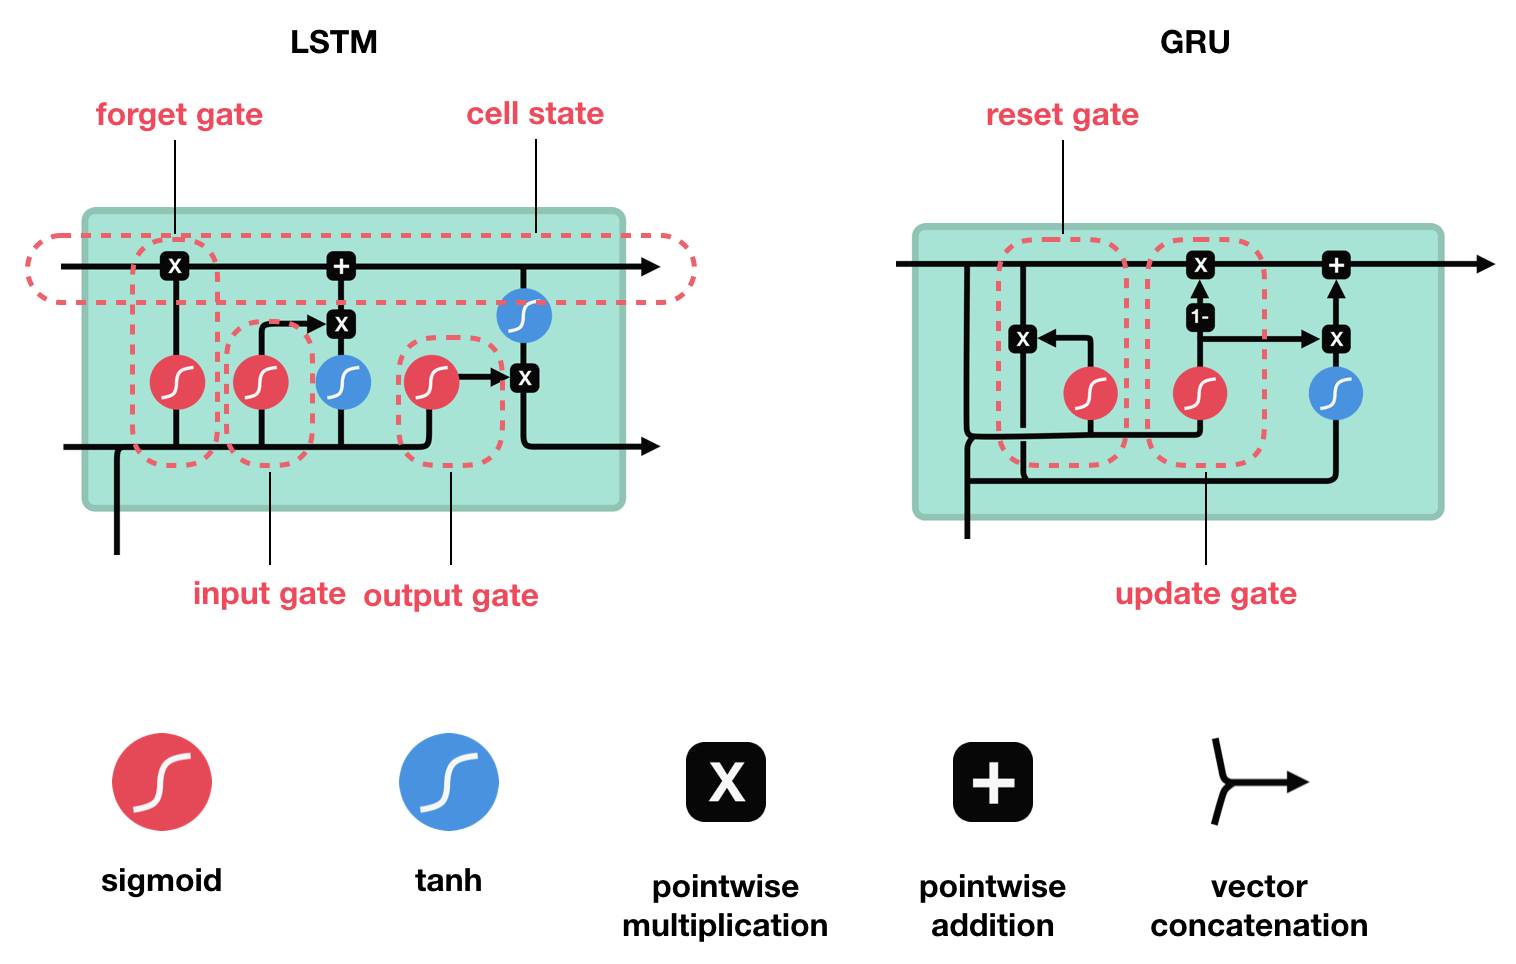
\includegraphics[width=0.80\textwidth]
    		{./Figs/10-portoes-rnns.png}
    	 	\caption{Arquitetura do modelo GRU.}\caption*{  Fonte: \cite{DLB}} \label{fig:gru-arch}}
    \end{figure}
    
    As redes GRU permitiram então a resolução de problemas com sequencias longas de dados, resolvendo o problema de memória a curto prazo. Então a maior dificuldade que poderia surgir ainda nos treinamentos supervisionados teria a ver com o overfitting, pelo qual foi proposta mais uma ferramenta para evitar que a rede memoriza-se além do desejado: o método \textit{dropout}.
    
    \subsubsection{Dropout} \label{sec:drop_fund}
    
    O método de \textit{Dropout} foi apresentado em \cite{dropout}, termo traduzido ao português na literatura como abandono, e propõe a remoção temporária de alguma célula da rede. 
    
    Em \cite{dropoutapp} foi aplicado \textit{dropout} no treino de uma rede neural, no qual, em cada época de treinamento são desligadas aleatoriamente algumas células da camada de entrada e algumas outras das camadas ocultas, sendo todas ligadas novamente no final da época. Com isso, em cada época do treino apenas uma amostra dos dados é processada por um subconjunto das células ocultas.  
    
    Esta técnica procura que a aleatoriedade da escolha de células em cada época induza uma redução na dependência entre elas as células no processo de ajuste, fazendo que cada unidade gere padrões que não dependam dos aprendidos pelas outras. No momento do teste, todos os pesos são multiplicados pela probabilidade da sua célula ter sido desligada. 
    
    Em \cite{dropoutapp} são obtidos bons resultados no treino da rede com \textit{dropout} quando, em cada época,  são desligadas 50\% das células em camadas ocultas e 20\% das células na camada de entrada.
    

    


    \chapter{Trabalhos relacionados} \label{cap:literatura}
  
Este capítulo descreve os principais trabalhos relacionados encontrados na literatura referenciada neste trabalho. A primeira seção cita a primeira referência literária encontrada na execução deste trabalho que realiza comparações de métodos de previsão de demanda. A segunda seção cita pesquisas relacionadas ao tema deste trabalho, a predição de demanda em restaurantes universitários, contendo estudos relacionados com uma parte dos métodos executados neste trabalho que são os modelos de redes neurais MLP, e o diferencial deste trabalho em relação aos outros é a inclusão de redes neurais recorrentes modernas, denominadas GRU, fundamentadas no tópico \ref{sec:GRU}. A última seção cita o maior volume de referências encontradas durantes as pesquisas de predição de demanda em geral, e que não corresponderam ao tema deste trabalho.

    \section{Trabalho de comparações de métodos de previsão de demanda.}
       \citeonline{Junior2007} Realiza um trabalho de comparação entre os métodos estocásticos (Método de suavização exponencial, modelos de Box-Jenkins) e modelos de aprendizado de máquina (Redes Neurais), ilustrados na Figuras \ref{fig: metodosPrevisaoDemanda}, os quais são usados para a previsão da demanda de produtos cosméticos distribuídos em séries temporais. Entre as Redes Neurais, encontramos redes do tipo \textit{feedforward} com o algoritmo de treino por \textit{backpropagation} que foi o principal foco no trabalho de previsão do R.U na Universidade Federal de Viçosa e na Universidade Estadual Paulista Júlio de Mesquita Filho, e que também fundamentou parte do desenvolvimento deste trabalho de predição no ICT Unifesp. Neste trabalho do autor, também são analisadas diversas medidas de performance preditivas e é feito uma análise comparativa final destas medidas entre os métodos citados.
    
    \section{Previsão de demanda em restaurantes universitários}
        No estudo estatístico feito por \citeonline{Landim2016}, foi analisada a correlação entre a temperatura e o consumo de refeições nos dias de vendas do restaurante universitário do campus ICT-Unifesp, sendo que os dados continham apenas uma pequena amostra das vendas do segundo semestre de 2016. Devido ao baixo volume de ocorrências, os dados foram submetidos à reamostragem via bootstrap. De acordo com os gráficos das amostras, identificou-se que a correlação mostrada nos gráficos da primeira metade do semestre e do período total do semestre formaram distribuições bimodais. Porém, na segunda metade do semestre formou-se uma distribuição unimodal. Portanto, concluiu-se que outras variáveis e outros modelos de análises deveriam ser utilizados para esta previsão de demanda.
        
        \citeonline{Lopes2008} faz o mesmo estudo deste cenário do ICT-Unifesp aplicado na Universidade Federal de Viçosa (UFV). Neste estudo, os dados utilizados foram somente o histórico de vendas do restaurante universitário, e nenhuma variável de ambiente foi coletada como temperatura, precipitação, número de alunos matriculados, etc. O algoritmo utilizado foi o \textit{Traincgp (Conjugate gradient backpropagation with Polak-Ribiere updates)} no software Matlab. Este algoritmo não envolve o cálculo das derivadas segundas das variáveis e converge ao mínimo da função quadrática em um número finito de iterações como cita o autor. Foram então considerados para cada nó da rede neural, o dia da semana (como segunda, terça, quarta, quinta e sexta) e cada camada dessa rede utilizando os 5 dias anteriores para cada nó (as 5 segundas anteriores, 5 terças anteriores e assim sucessivamente) e, por fim, obtido um modelo pela rede que apresentou erro máximo de 3. A rede neural aplicada neste trabalho é representada na Figura \ref{fig:mlp-lopes}.
        
        \begin{figure}[h]
        \center{
        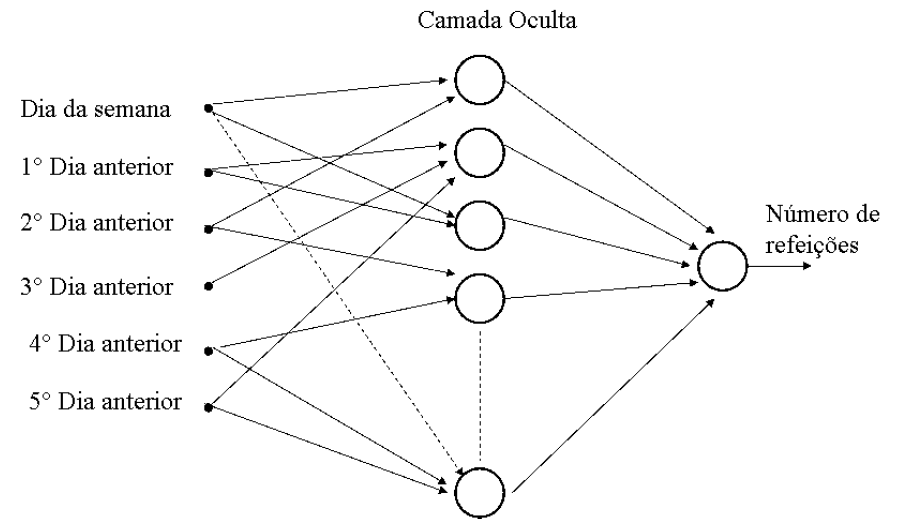
\includegraphics[width=\textwidth]
        {./Figs/15-rna-lopes.png}
        \caption{Rede Neural Perceptron de Múltiplas Camadas.}\caption*{  Fonte:\cite{Lopes2008}.}\label{fig:mlp-lopes}}
        \end{figure}
        
        \citeonline{Rocha2011} também realiza o estudo de demanda no restaurante universitário da Universidade Estadual Paulista Júlio de Mesquita Filho (UNESP), novamente com os métodos de redes neurais artificiais com backpropagation e utilizando apenas como fonte de dados (o histórico numérico das vendas realizadas), e outras variáveis intermediárias obtidas a partir deste, como médias de subconjunto de observações (médias de segundas-feiras). A única variável de ambiente coletada foi o número de feriados próximos à observação de venda. No estudo do total de dias analisados, verifica-se que em 73\% (187 dias), o método de média simples propiciou um maior erro em relação à RNA, que por sua vez ocasionou um erro maior nos 23\% (69 dias) restantes.Em se tratando de menor desperdício, observa-se que a RNA apresenta erros maiores que 50 refeições em 13 dias, enquanto o método da média simples apresenta erros maiores que 50 refeições em 58 dias, concluindo-se então que o método de RNA foi bem mais eficiente do que o cálculo de média simples utilizado pela administração do restaurante universitário. A Figura \ref{fig:rnaRocha} apresenta um esquema da rede  neural aplicada nesse trabalho. 
        \begin{figure}[h]
        \center{
        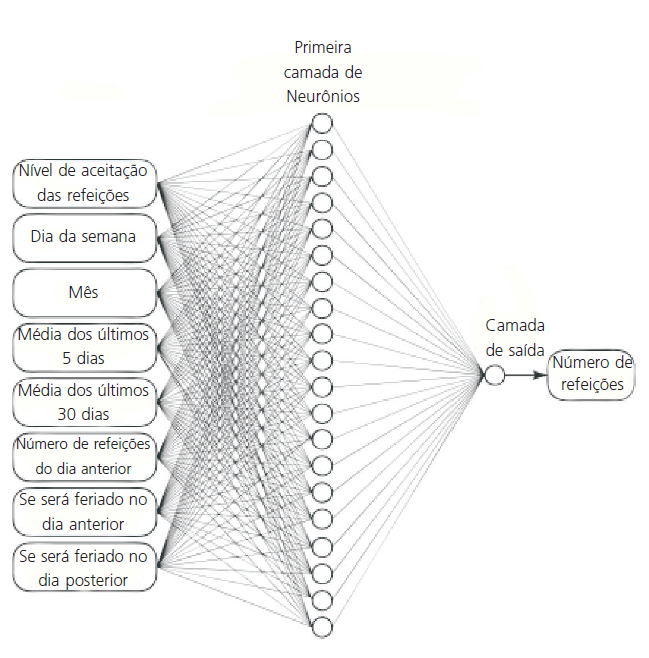
\includegraphics[width=0.8\textwidth]
        {./Figs/16-rna-rocha.png}
        \caption{Rede Neural Perceptron de Múltiplas Camadas}\caption*{ Fonte: \cite{Rocha2011}} \label{fig:rnaRocha}}
        \end{figure}
        
        Tanto o modelo apresentado em \cite{Rocha2011} quando em \cite{Lopes2008} possuem uma única camada oculta. 
      
    \section{Previsão de demanda em outros ambientes}
        \citeonline{RUAS2012} faz uma análise de previsão de demanda de energia elétrica no estado do Paraná, entre os anos de 2004 e 2006, utilizando redes neurais artificiais e máquinas de vetores de suporte. Apesar de não ser o mesmo exemplo do cenário do restaurante universitário do ICT-Unifesp, temos a distribuição dos dados de consumo coletados como uma série temporal. Nesta pesquisa de previsão de demanda de energia elétrica foi utilizada uma rede parcialmente recorrente de Elman, que permite a previsão de um passo de tempo à frente. Para que seja possível realizar a previsão para vários pontos à frente, é necessário utilizar os valores já previstos, ou seja, a saída da rede, como entradas da mesma.
        
        \citeonline{Almeida2013} analisa um cenário semelhante de demanda de energia elétrica, porém utilizando-se técnicas de previsão de demanda com Rede Neural Artificial do tipo Multilayer Perceptron combinado com lógica fuzzy que permite colocar variáveis de temperatura (entre outras) em um conjunto de regras que impactam no problema.
        
        \citeonline{Silva2010} também aplica técnicas de redes neurais para previsão de demanda de energia elétrica, com o estudo de variáveis climáticas, porém através de um modelo de MAPA SOM - (Self-Organizing Map) que é um tipo de rede neural desenvolvido para reconhecimento de padrões. Apesar de ser um modelo não supervisionado, o modelo é ideal para organizar as principais variáveis impactantes e descartáveis na previsão. O mapa som utilizado pelo autor apresenta os dados associados aos seus neurônios de forma que padrões similares encontram-se em neurônios contíguos, tendo uma organização topológica. Deste modo é possível se extrair relações abstratas entre as variáveis do vetor de dados através da sua posição nos mapas componentes, que por meio de uma escala de cores mostram a quantidade de uma variável específica em cada neurônio do mapa.
    
\chapter{Metodologia} \label{cap:metodos}


% ISSO aqui é metodologia
%Como foi evidenciado nas comunicações com a gestão do restaurante, a análise utilizada para se prever as refeições é produzir no dia da semana, como por exemplo uma segunda-feira, o consumo do mesmo dia da semana anterior (segunda-feira anterior) com acréscimo de uma margem de erro. Em geral, de acordo com o restaurante, todos os dias o mesmo trabalha com um erro e um descarte de 30\% das refeições que são trazidas e consumidas ao campus. Estima-se então que no período de 2011 - 01/08/2018 os estabelecimentos tenham tido um prejuízo de R\$1.885.938,40, e de 30\% de R\$78.386,85 no atual período de 01/08/2018 - 31/10/2018 totalizando o montante  R\$1.964.325,25. Aproximadamente 2 milhões de reais em prejuízo acumulado desde 2011.



% A obtenção dos dados do R.U do ICT Unifesp se encontra em formato de série temporal, ou seja, o consumo e vendas de refeições no R.U se distribuem em função do tempo, pelos dias letivos da universidade.
 
 
 % O cenário deste estudo analisa a sazonalidade da frequência de alunos do ICT - UNIFESP, inferida pelas grades semestrais de suas disciplinas, que consequentemente inferem na sazonalidade de consumo de refeições dentro do restaurante universitário. 
 
 
 
 
   Neste Capítulo é descrita a metodologia experimental deste trabalho, a qual consiste nos seguintes passos:
    \begin{itemize}
        \item Coleta de dados endógenos e exógenos.
        \item Transformação de cada registro de dado endógeno (os dados de consumo e vendas), em uma série temporal com intervalo de cinco dias anteriores.
        \item Análises exploratórias dos conjuntos de dados endógenos e exógenos com o conjunto de dados a serem previstos.
        \item Construção e treino dos modelos exclusivamente endógenos e dos modelos mistos, duplicados em duas fases experimentais com diferentes domínios temporais.
        \item Análises comparativas dos resultados dos modelos.
    \end{itemize}
    
    \section{Área de estudo}
       A área de estudo deste trabalho é o restaurante universitário do Instituto de Ciência e Tecnologia da Unifesp (ICT-Unifesp) em São José dos Campos. O campus do ICT foi inaugurado no ano de 2007 visando suprir as demandas científicas e tecnológicas da região do Vale do Paraíba. A Figura \ref{fig:RU_foto} apresenta um dia comum de utilização do espaço físico do restaurante unuversitário do ICT.
        
        \begin{figure}[H]
        	\center{
        	    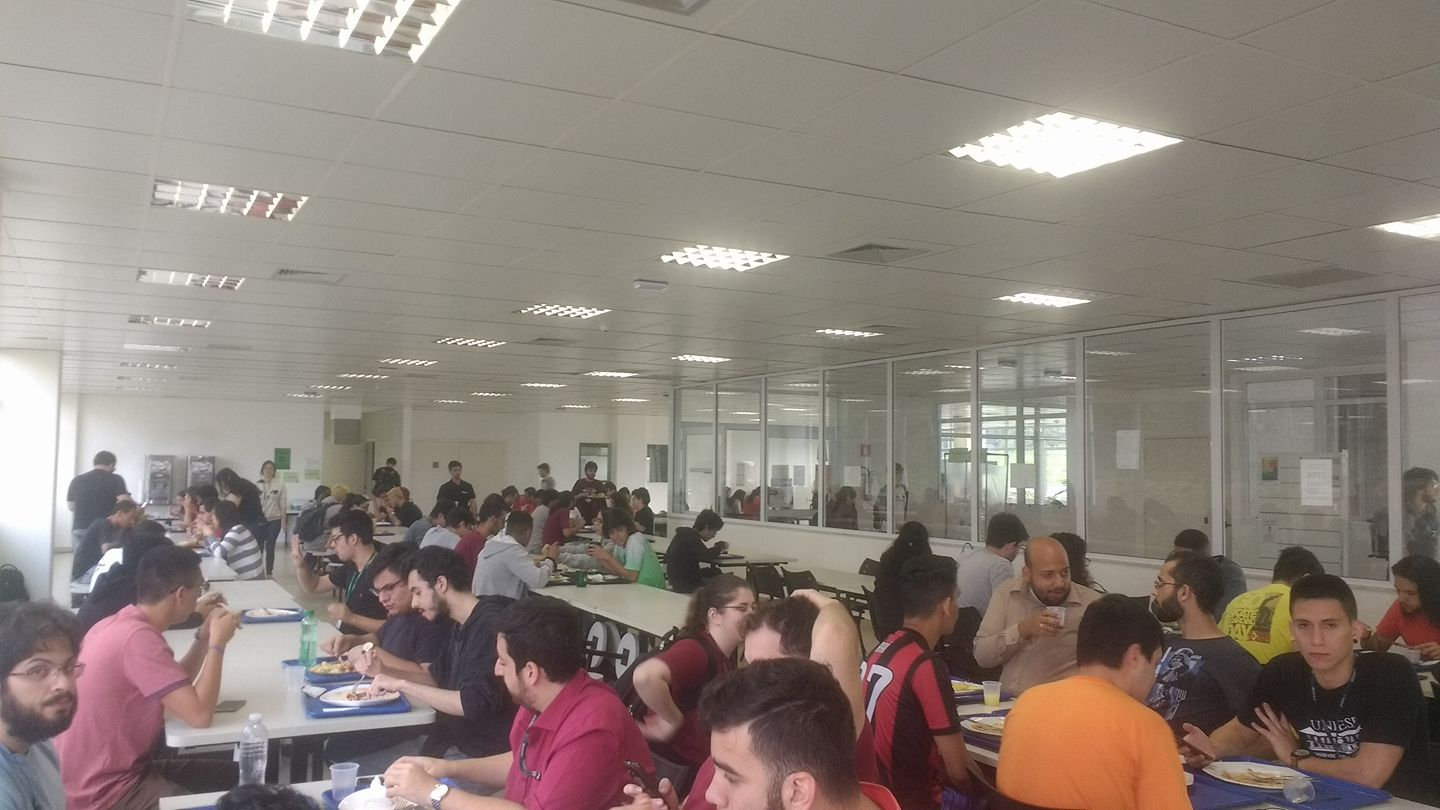
\includegraphics[width=0.7\textwidth]{./Figuras/ru_unifesp.jpg}
        	    \caption{Restaurante Universitário do ICT-Unifesp}\label{fig:RU_foto}
        	     }
        \end{figure}
    
    \section{Descrição dos dados}

    Este trabalho fará uso de dois tipos de dados, endógenos e exógenos, os quais são descritos a seguir. 
            
    Dados endógenos:  são os dados do domínio de predição neste caso. Para este problema, são as quantidades diárias de  refeições consumidas no almoço e no jantar do Restaurante Universitário (RU) do ICT-Unifesp, quantificada diariamente pela número de alunos que passam no ponto de acesso, a catraca. 
    Também são considerados dados endógenos a quantidade diária  de \textit{tickets} de refeição vendidos pelo Restaurante. Em ambos casos, as informações são tidas dos dias letivos.   Esses dados são transformados em entrada de redes neurais, em formato de série temporais.
            
    Dados exógenos: são todos os outros dados fora do domínio de predição. Para este problema, são  parâmetros derivados das datas das observações, como por exemplo o dado categórico que representa o dia da semana (segunda-feira à sexta feira), e os dados climáticos.
    
    \section{Obtenção e tratamento dos dados}
        A obtenção dos dados é realizada por meio de duas fontes distintas, sendo os dados endógenos inteiramente fornecidos através do setor de tecnologia da informação do ICT Unifesp, parte dos dados exógenos da data de registro dos dados endógenos coletados, e a parte restante dos dados exógenos, os dados climáticos, são obtidos através da uma estação meteorológica mais próxima ao ICT Unifesp, localizada na cidade de Taubaté-SP.
        
	    \subsection{Dados endógenos} \label{subsec:coleta_endogenos}
        	Os dados históricos de consumo no restaurante foram retirados do atual sistema banco de dados de refeições subsidiadas do Hospital São Paulo, que gerencia os dados dos refeitórios de todos as unidades da Unifesp. Apenas alguns funcionários autorizados têm acesso ao banco de dados da instituição, portanto para coletar tais dados o presente trabalho obteve uma autorização com a direção do campus ICT-Unifesp. Foram solicitados  os dados de consumo apenas para os discentes de graduação, visto que  o banco de dados ainda possui as informações de consumo de docentes, alunos de pós-graduação e visitantes, porém claro com menor relevância em termos quantitativo. Além disso, o padrão de consumo destes outros estratos do meio acadêmico pode influenciar  o processo de predição das demandas trazendo tendências diferentes. Na tabel \ref{table:dadosrestaurante}.
    
        	\begin{table}[!ht]
        	    \centering
        	    \caption{Formato original dos dados originais obtidos pelo restaurante universitário}
                \rowcolors{2}{gray!25}{white}
                \begin{tabular}{l|l|l}
                    \hline
                    DATA                  & (19/12/2017) & (18/12/2017) \\ \hline
                    VENDAS CAFÉ           & 0            & 0            \\
                    VENDAS ALMOÇO         & 24           & 71           \\
                    VENDAS JANTAR         & 0            & 0            \\
                    VENDAS REFEIÇÃO      & 24           & 71           \\
                    TOTAL VENDAS          & 24           & 71           \\
                    ENTR. CAFÉ            & 0            & 0            \\
                    ENTR. ALMOÇO          & 42           & 70           \\
                    ENTR. JANTAR          & 3            & 24           \\
                    TOTAL ENTR. REFEIÇÃO & 45           & 94           \\
                    TOTAL ENTRADA         & 45           & 94           \\ \hline
                \end{tabular}
               
                \label{table:dadosrestaurante}
            \end{table}
            
            Após a coleta, os dados de consumo do restaurante foram transformados em um processo de aproximação por uma série temporal, para um intervalo de cinco dias, e em cada registro de venda  acrescentados cinco novos atributos contendo os valores passados, deste mesmo atributo, em um intervalo de cinco dias anteriores. Este processo adapta o conjunto de dados para o processo de memorização das entradas, estruturando o formato compatível de leitura de dados nos modelos de redes neurais aplicados.
            
            A Tabela \ref{table:transformacaodadosrestaurante} exemplifica a nova estrutura de um registro de dado do restaurante, com um intervalo temporal de cinco dias anteriores. Nota-se que o valor de consumo da data 20/04/2017 foi removido do conjunto de dados, por se tratar o valor supervisionado a ser previsto, dado que o processo de aprendizado das redes neurais utilizam apenas dados no passado, a partir de um dia anterior.
            
            \begin{table}[!ht]
                \centering
                \rowcolors{2}{gray!25}{white}
                \begin{tabular}{l|l}
                \hline
                    DATA                  & (19/12/2017) \\ \hline
                1 DIA ANTERIOR    & 500        \\
                2 DIAS ANTERIORES & 00                            \\
                3 DIAS ANTERIORES & 300                            \\
                4 DIAS ANTERIORES & 200                            \\
                5 DIAS ANTERIORES & 100                          \\ \hline 
                \end{tabular}
                \caption{Transformação dos registros do restaurante em uma série temporal.}
                \label{table:transformacaodadosrestaurante}
            \end{table}
           
        \subsection{Dados exógenos} \label{subsec:coleta_exógenos}
            Os dados exógenos correlacionados com o consumo se dividem em dois tipos principais, dados climáticos coletados de estações meteorológicas próximas ao ICT-Unifesp, e dados derivados das datas dos registros de consumo.
    
      	 Em relação as variáveis climáticas utilizadas como dados exógenos, foram considerados parâmetros que possam afetar o consumo de refeições de forma indireta, como temperatura média ambiente, pressão atmosférica, umidade e velocidade do vento. Tais parâmetros podem ser obtidos de forma gratuita pelo BDMEP - Banco de Dados Meteorológicos para Ensino e Pesquisa, pertencente à instituição pública INMET - Instituto Nacional de Meteorologia, pertencente ao Ministério da agricultura, pecuária e abastecimento. É necessário um cadastro na plataforma do INMET \footnote{\url{http://www.inmet.gov.br/portal/index.php?r=bdmep/bdmep}} para a obtenção dos dados. A instituição contêm dados registrados de forma digital desde 1961 no país inteiro, os dados históricos referentes a períodos anteriores a 1961 ainda não estão em forma digital e, portanto, estão indisponíveis no BDMEP. Importante ressaltar que o BDMEP leva 90 dias para registrar cada nova data. 
            	
     	  Além dos dados ambientais, também foram gerados dados exógenos a partir dos dados de consumo coletados. A informação de data contida nos índices dos registros dos dados endógenos, foi derivada em diversas informações que representam o comportamento de consumo em relação à sazonalidade da frequência dos alunos influenciada pelas agendas de atividades acadêmicas.\\
            	Os seguintes parâmetros foram definidos:
            	\begin{itemize}
            	    \item Semestre 1 ou 2 em formato categórico e binário;
            	    \item Dia da semana em formato categórico e binário;
            	    \item Distancia em dias até o registro anterior e posterior;
            	    \item Avanço do semestre em escala percentual;
            	    \item Avanço do mês em escala percentual.
            	\end{itemize}
            	
            	O consumo distribuído em uma janela de cinco dias para entrada nas redes MLP seguiu padrão semelhante com os trabalho de previsão de demanda em R.U realizados por \citeonline{Lopes2008} e \citeonline{Rocha2011}, ilustrado na Figura \ref{fig:mlp-lopes}. Por fim, a Tabela \ref{table:dataset_final} representa o conjunto de dados estruturados e preparados para o processo de divisão em domínios de treino, validação e teste para o treino dos modelos.

       \begin{table}[!ht]
            \centering
            \rowcolors{2}{gray!25}{white}
            \begin{tabular}{c|c|c} \hline
                \multicolumn{3}{c}{ Estrutura final do conjunto de dados indexados por data: } \\
                \hline
                identificador &	nome da variável					&tipo de variável\\ 
                \hline
                0&	SEMESTRE\_1					&int64 \\
                1&	SEMESTRE\_2					&int64\\
                2&	SEGUNDA						&int64 \\
                3&	TERCA						&int64 \\
                4&	QUARTA						&int64 \\ 
                5&	QUINTA						&int64 \\ 
                6&	SEXTA						&int64 \\ 
                7&	DISTANCIA\_DIA\_ANTERIOR	&	int64 \\ 
                8&	DISTANCIA\_DIA\_POSTERIOR	&	int64 \\
                9&	PERC\_CONCLUSAO\_SEM		&	float64 \\
                10&	PERC\_CONCLUSAO\_MES		&	float64 \\
                11&	PRESSAO\_ATMOSFERICA		&	float64 \\
                12&	TEMPERATURA					&float64 \\ 
                13&	UMIDADE						&int64 \\
                14&	VENTO						&float64\\ 
                15&	VENDAS\_ALMOCO				&int64 \\
                16&	VENDAS\_ALMOCO\_1			&	int64 \\ 
                17&	VENDAS\_ALMOCO\_2			&	int64 \\
                18&	VENDAS\_ALMOCO\_3			&	int64\\ 
                19&	VENDAS\_ALMOCO\_4			&	int64 \\
                20&	VENDAS\_ALMOCO\_5			&	int64 \\ 
                21&	ENTR\_ALMOCO				&	int64\\
                22&	ENTR\_ALMOCO\_1				&int64 \\
                23&	ENTR\_ALMOCO\_2				&int64 \\
                24&	ENTR\_ALMOCO\_3				&int64 \\ 
                25&	ENTR\_ALMOCO\_4				&int64 \\
                26&	ENTR\_ALMOCO\_5				&int64 \\
                27&	ENTR\_JANTAR				&	int64 \\ 
                28&	ENTR\_JANTAR\_1				&int64\\
                29&	ENTR\_JANTAR\_2				&int64 \\ 
                30&	ENTR\_JANTAR\_3				&int64 \\ 
                31&	ENTR\_JANTAR\_4				&int64 \\
                32&	ENTR\_JANTAR\_5				&int64\\
              \hline
            \end{tabular}
            \caption{Estrutura final do conjunto de dados indexados por data}
            \label{table:dataset_final}
        \end{table}
        Por fim, a Tabela \ref{table:dataset_final} representa o conjunto de dados estruturados e preparados para o processo de divisão em domínios de treino, validação e teste para o treino dos modelos.
        
	\subsection{Pré-processamento}
        Na etapa de pré-processamento é realizada a transformação dos dados endógenos em séries temporais, de comprimento de cinco dias, normalização com remoção de \textit{outliers}, e aplicação de escala 0 a 1, para que todos os dados correspondam à um mesmo domínio de aprendizado. Após a conclusão destas etapas, o conjunto de dados foi preparado para as fases experimentais 1 e 2, que realizaram uma divisão do conjunto final de dados em intervalos temporais distintos. Apesar da distribuição dos dados se apresentarem em datas em função do tempo se classificando em um modelo de série temporal, assume-se a hipótese que o comportamento dos mesmos também é impactado por relações causais com outros variáveis exógenas, como recesso acadêmico, feriados, eventos, precipitações intensas que causam trânsito local e impactam na logística e frequência do público, entre outras variáveis de causas menos aparentes
    
        \subsection{Tratamento dos dados para entrada nos modelos}
         	Os dados endógenos, após estruturados na tabela final do conjuntos de dados, passam pelas seguintes transformações:
         	\begin{itemize}
                \item	Calculo do desvio padrão de cada vetor de atributos, e normalização dos valores máximos para o teto de 3x o desvio padrão, e mínimo de 0; 
                \item	Transformação dos dados em escala de 0 e 1.
            \end{itemize}
            Os dados exógenos não passam pela transformação em série temporal, portanto os mesmos foram tratados de acordo com os passos:
            \begin{itemize}
                \item	Transformação dos dados em escala de 0 e 1;
                \item	Os parâmetros categóricos binários (dias da semana e semestre) já estão escalados por serem categorias binárias.
            \end{itemize}
    	\subsection{Fases Experimentais} \label{subsec:fases_experimentais}
            O processo experimental foi realizado em dois roteiros distintos de divisão do domínio temporal do conjunto de dados, e os resultados obtidos entre as duas fases foram comparados.
            
            O conjunto de dados contemplando o período de 2017 a 2019, foi dividido em conjunto de treino, validação e teste da seguinte maneira: 
            
            \paragraph{1º Fase com validação no 1º semestre de 2018 e teste no 1º semestre de 2019}
                Neste roteiro, o semestre de validação que compõe o conjunto de dados para o treino \textit{backpropagation} das redes neurais contempla o primeiro semestre de 2018 e o conjunto de teste contempla o primeiro semestre de 2019.
                Os dados de 2017 contemplando o 1º e 2º semestre, e 2018 contemplando o 2º semestre, foram usados para treino. Os resultados obtidos nesta divisão foram usados para validar a hipótese de que os modelos aprendem especificamente a sazonalidade de consumo no primeiro semestre, se saindo melhor nos testes realizados no primeiro semestre de 2019, em comparação aos outros modelos treinados com validação no ano todo de 2018.
                Portanto, o conjunto de dados da primeira fase contempla o seguinte domínio:
            \begin{itemize}
                    \item Conjunto de treino dos modelos, contemplando o primeiro e segundo semestre de 2017, e segundo semestre de 2018;
                    \item Conjunto de validação dos modelos, contemplando o primeiro semestre de 2018;
                    \item Conjunto de teste dos modelos, contemplando o primeiro semestre de 2019.             
            \end{itemize}
            
            \paragraph{2º Fase com treino em 2017, validação em 2018 e teste em 2019}
                Nesta fase, os conjuntos foram divididos conforme sua descrição e o melhor modelo encontrado passa por uma última etapa de teste no domínio da primeira fase (teste somente no primeiro semestre de 2019).
                As métricas obtidas neste teste foram comparadas com o melhor modelo da primeira fase.
    
    \section{Definição e treino dos modelos}
            %\paragraph*{Sobre a necessidade de implementar modelos mistos}
                No conjunto de dados deste trabalho, os dados obtidos se dividem em dados temporais e endógenos (tal que cada registro de consumo e venda trás a informação de seu domínio em um intervalo temporal de cinco dias anteriores) e dados discretos e exógenos, sendo variáveis categóricas de data para cada registro, e variáveis climáticas.
                
                Portanto foi necessária a implementação de modelos específicos para entradas temporais e modelos específicos para as entradas discretas.
                Para a saída final foi implementado um comitê de redes neurais endógenas e exógenas, com um neurônio perceptron na saída, recebendo os dois valores dos modelos endógenos e exógenos para a regressão das saídas das duas redes ao valor que será a predição do consumo.
         	\paragraph{Modelos endógenos}
         	\begin{itemize}
                \item	Desenvolvimento das redes perceptron de baixa profundidade para avaliar o aprendizado da rede;
                \item	Aumento da profundidade da rede e avaliar as mudanças da função de perda RMSE; 
                \item	Implementação e avaliação dos modelos com redes recorrentes GRU, conforme a Figura. \ref{fig:gru-arch} que são especialmente desenvolvidos para o aprendizado com memorização de dados, e no caso deste trabalho, podem memorizar as sazonalidades semanais de consumo (em um intervalo de cinco dias).
            \end{itemize}
            \paragraph{Modelos Mistos : Endógenos e Exógenos}
                \begin{itemize}
                    \item Para os dados temporais (consumo e venda) utilizou-se os melhores modelos endógenos dos experimentos anteriores para as entradas endógenas. 
                    \item Para os dados discretos e categóricos adaptou-se a entrada destes dados para rede perceptron
                    \item  Concatenou-se a saída das duas redes neurais em um perceptron criando um comitê de redes neurais para obter a saída final prevista.
                \end{itemize}
            
	\subsection{Hiper parâmetros : Função de ativação e otimizador}
        Conforme fundamentado no Capítulo \ref{cap:teoria} na Seção \ref{sec: perceptron}, a função de ativação dá a capacidade do perceptron, quando conectado em rede, de resolver problemas lineares e não lineares, agregando adaptação e improviso ao resolver programas que não estão contidos em seus dados de alimentação.
        Portanto para as camadas ocultados das redes neurais MLP desenvolvidas será aplicada a função ReLu e para o neurônio de saída será aplicada a função linear, e o otimizador de treino realiza a função de otimizar o tempo de convergência do reajuste dos pesos à valores ideais, sendo escolhido o otimizador ADAM com taxa de aprendizado definido em 0,001.

    \section{Teste e Métricas de avaliação}
       As principais métricas de avaliação dos modelos são a Raiz do Erro Quadrático Médio ou em inglês \textit{Root Mean Squared Error} (RMSE), O coeficiente de correlação de Pearson (R), e o coeficiente "chi-quadrado" definido como $R^2$. Estas métricas estatísticas foram utilizado nas etapas de teste para avaliar a proximidade das predições do modelo com o comportamento real de consumo. As equações \ref{eq:RMSE} e \ref{eq:Pearson} apresentam a formulação para o RMSE e o coeficiente de Pearson (R), respectivamente.
       
       \begin{equation}
           RMSE = \sqrt{\frac{1}{n}  \sum_{i=1}^n (x_i^{est} - x_i^{obs})^2}
           \label{eq:RMSE}
       \end{equation}
       
       \begin{equation}
           R = \frac{\frac{1}{n}  \sum_{i=1}^n (x_{est} - \bar{x}_{est}) * (x_{obs} - \bar{x}_{obs})}{\sigma_{est} * \sigma_{obs} }
           \label{eq:Pearson}
       \end{equation}
       
       Onde “est” são os valores estimados; “obs” são os valores reais; n é o numero de amostras ; $\sigma$ é o desvio padrão; R é a correlação linear; $\bar{x}$ é a média de x. Avaliou-se também os erros positivos e negativos entre os valores previstos e reais, para representar quantas refeições seriam descartadas e quantas estariam em falta se a produção de refeições fosse de acordo com as predições do modelo.
       
  % ----------------------------------------------------------
  % \chapter{METODOLOGIA}
  % ----------------------------------------------------------
    \chapter{Resultados} \label{cap:resultados}

\TEXTO{Este capítulo descreve os principais resultados experimentais obtidos durante esta pesquisa. Como descrito no capítulo anterior, os experimentos foram conduzidos em duas fases. Contudo, optou-se por apresentar, neste capítulo, apenas os principais resultados obtidos. Um sumário dos demais resultados estão disponíveis no Anexo XX deste documento.}

\TEXTO{Antes de apresentar os resultados, as primeiras seções introduzem a organização dos dados, um breve análise das variáveis e o protocolo experimental, respectivamente.}

\section{Organização do conjunto de dados}
\TODO{descrever, nessa seção, como os dados foram organizados em treino, validação e teste}

    O procedimento de coleta de dados foi realizado de acordo com a metodologia da subseção \ref{subsec:coleta_endogenos} para os dados endógenos, e de acordo com os passos da subseção \ref{subsec:coleta_exógenos} foram obtidos os dados exógenos. 
    Ambos os conjuntos de dados coletados foram estruturados conforme a tabela \ref{table:dataset_final}, contendo um intervalo temporal de registros, desde a data 2017-04-12 (12 de abril de 2017) para o primeiro registro até a data 2019-12-16 (16 de dezembro de 2019) para o último registros, totalizando 514 registros de consumo de refeições em dias letivos.
    
    Conforme a metodologia definida na subseção \ref{subsec:fases_experimentais} este conjunto de dados com o total de 514 registros, foi duplicado para 2 fases experimentais distintas, cada uma com sua organização específica do conjunto de dados.
    
    O conjunto de dados da primeira fase experimental foi organizado de acordo com a figura \ref{fig:case1_timeline}, esta fase tem o conjunto de validação contemplando exclusivamente o primeiro semestre de 2018, indicando uma hipótese de que o primeiro semestre de 2018 tivesse um movimento de consumo e vendas semelhantes ao primeiro semestre de 2019, tal que esta fase seria a ideal para testes envolvendo só o primeiro semestre do conjunto de testes.

    \begin{figure}[htb]
        	\center{
        		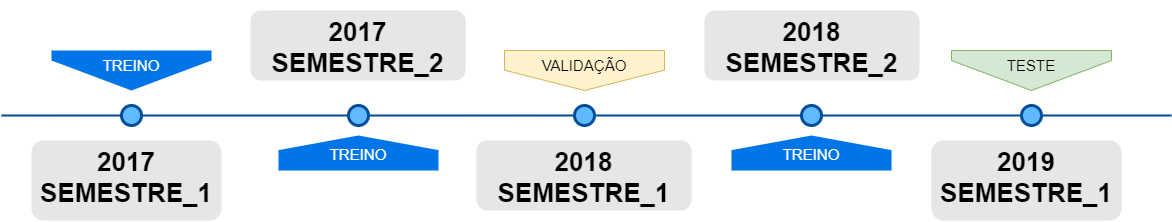
\includegraphics[width=1.0\textwidth]{./Figuras/resultados/case1_timeline.png}
        	
        	\caption{Domínio temporal da 1a fase} \label{fig:case1_timeline} }
        \end{figure}
    E na segunda fase o conjunto de dados foi organizado de acordo com a figura \ref{fig:case2_timeline}, e como esta fase teve um conjunto de validação contemplando 1 ano letivo inteiro, o de 2018, os experimentos de testes dos modelos nesta fase contemplaram o ano todo de 2019.
    
    \begin{figure}[H]
        	\center{
        		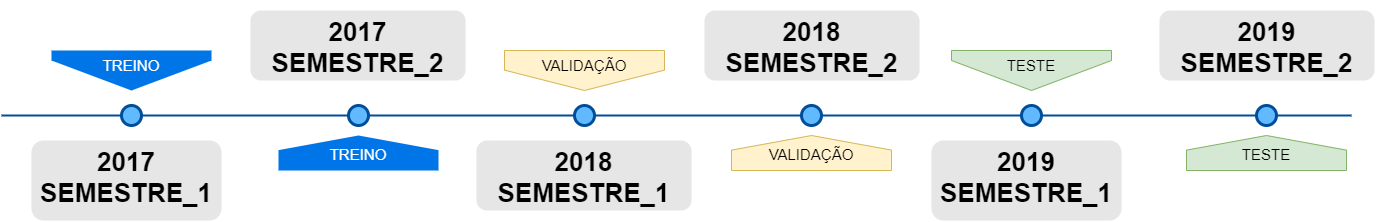
\includegraphics[width=1.0\textwidth]{./Figuras/resultados/case2/case2_dominio.png}
        	
        	\caption{Domínio temporal da 2a fase} \label{fig:case2_timeline} }
        \end{figure}
   
    \paragraph{Dificuldades encontradas e resolvidas}
    A primeira dificuldade encontrada nos experimentos foi um comportamento anômalo do gráfico de previsão, a linha azul na figura \ref{fig:pandas_wrong_indexing} representa uma previsão do modelo que obteve os melhores resultados na primeira fase, e a linha vermelha neste mesmo gráfico representando os valores reais de consumo do primeiro semestre de 2019 também foi anômala. E após uma análise foi descoberto que os registros continham um erro na indexação por data, trocando datas (dia por mês e mês por dia), após a correção da indexação os gráficos de consumo real e previsão produziram resultados melhores e dentro do formato esperado, conforme a figura \ref{fig:pandas_correct_indexing}.
    
    \begin{figure}[htb]
    	\center{
    		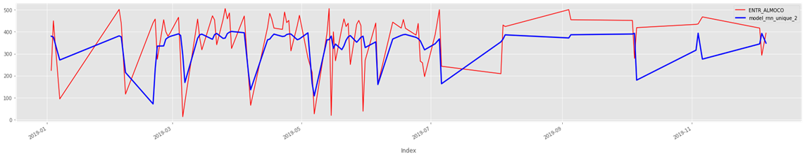
\includegraphics[width=1.0\textwidth]{./Figuras/resultados/pandas_wrong_indexing.png}
    	
    	\caption{Resultado do modelo RNN\_ENDO\_2 obtido sobre o conjunto de dados aleatoriamente ordenado sobre o tempo} \label{fig:pandas_wrong_indexing} }
    \end{figure}
    
    \begin{figure}[htb]
    	\center{
    		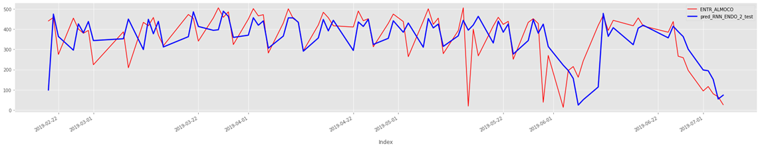
\includegraphics[width=1.0\textwidth]{./Figuras/resultados/pandas_correct_indexing.png}
    	
    	\caption{Resultado do modelo RNN\_ENDO\_2 obtido sobre o conjunto de dados com ordenação corrigida \label{fig:pandas_correct_indexing} }}
    \end{figure}
              
\section{Avaliação das Variáveis}
\TODO{use essa seção se quiser detalhar algo sobre as principais variáveis consideradas, caso contrário, pode excluí-la. Ajuste o texto inicial do capítulo se resolver remover essa seção}

    \paragraph{Estimativas de consumo do restaurante}
        A análise da técnica de estimação de consumo, realizada pela análise subjetiva do consumo da semana anterior, foi feita com o cálculo de 30\% de produção acima do consumo do 5o dia anterior. É possível notar que este método de estimativa é feito para tolerar descartes devido à multa contratual para falta de refeições e que a produção de 30\% de refeições acima do consumo da semana anterior, na figura  \ref{fig:ru_pred} produz um comportamento linear, na linha azul, distante do comportamento real de consumo na linha vermelha. Apesar da estimativa seguir as tendências de quedas e aumento de consumo, a figura \ref{fig:ru_pred_scatter} do gráfico scatter gerado entre a estimava do R.U e o consumo real no ano de 2019, demonstra que a regressão linear (representada pela linha vermelha no gráfico scatter) tem o eixo totalmente descentralizado com a função identidade da estimativa ideal (representada pela diagonal imaginária formada entre a origem do gráfico e o vértice superior direito), gerando também um erro maior do que 30\% no somatório total de refeições descartadas no semestre, ocasionado pelo comportamento oscilatório do consumo, conforme a tabela \ref{table:case2_rupred}.
        {
            \begin{center}
            \begin{minipage}[c]{1.0\textwidth}
                \begin{figure}[H]
                    \center{                    
                        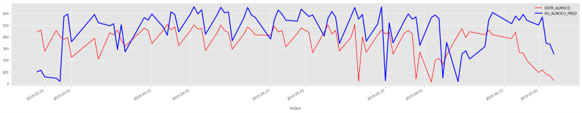
\includegraphics[width=\textwidth]{./Figuras/resultados/case1_ru_pred.png}
                        \caption{Estimativa do restaurante para o ano de 2019} \label{fig:ru_pred} 
                    }
                \end{figure}
            \end{minipage} \hfill %
            
            \begin{minipage}[c]{0.8\textwidth}
                \begin{figure}[H]
                    \center{                    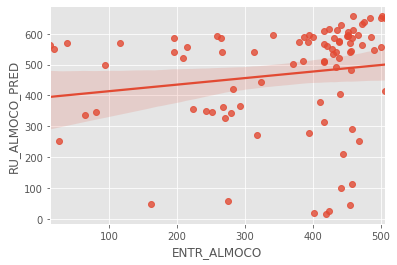
\includegraphics[width=\textwidth]{./Figuras/resultados/case1_ru_pred_scatter.png}
                    \caption{Gráfico scatter da estimativa de consumo do restaurante para o ano de 2019} \label{fig:ru_pred_scatter} }
                \end{figure} 
            \end{minipage} 
            \end{center}
            
            \begin{table}[!ht]
            \centering
            \caption{Métricas da estima de consumo do restaurante para o ano de 2019}
            \label{table:case2_rupred}
            \rowcolors{2}{gray!25}{white}
                \begin{tabular}{|c|c|}
                \rowcolor{gray!50}
                \hline
                \multicolumn{2}{c}{Consumo com margem 30\% acima do 5o dia anterior}\\ \hline     
                TOTAL DE REFEIÇÕES CONSUMIDAS & 58653  \\
                TOTAL DE REFEIÇÕES ESTIMADAS & 76262 \\ 
                CORRELAÇÃO (r)&  0.40067947341844423 \\
                P-value & 2.0845891721642294e-08\\
                RMSE & 191.7620291511743 \\
                SOMA DOS ERROS POSITIVOS & 23412 \\
                SOMA DOS ERROS NEGATIVOS & -5803 \\
                ERRO ABSOLUTO MEDIANO & 133.0 \\
                ERRO ABSOLUTO PERCENTUAL MEDIO & 205.61135949728225\% \\  \hline 
                \end{tabular}
            \end{table}
        }
    \subsection{Análise das variáveis endógenas}
        As variáveis endógenas são os parâmetros temporais de entrada nos modelos MLP e GRU, correspondentes ao domínio de consumo no restaurante.
         % \newpage
        \paragraph*{Consumo do dia vigente em relação às vendas de tickets do dia anterior}
        É possível notar na figura \ref{fig:case1_consumo_vendas_almoco} que as vendas de ticket no período de almoço apresentaram comportamento diferente no ano de 2017 em comparação aos anos seguintes devido à uma limitação imposta pelo restaurante, a partir de 2018, que os alunos comprassem apenas 2 tickets por dia. Possivelmente esta limitação foi dada para aproximar o comportamento de consumo de 1 até 2 dias seguintes à vendas de tickets no dia vigente, esta limitação pode ser interpretada como método de auxílio à gestão para a produção de refeições e para o tratamento de desperdício.
	        
        Mesmo com o valor outlier de 2000 vendas em um único dia, e com a nova limitação de compras de tickets a partir de 2018, o consumo no horário de almoço está fortemente relacionado com as vendas de tickets no período do almoço de 1 dia anterior e nota-se que os alunos se adaptaram à limitação imposta para utilização dos tickets com prazo de validade de 2 dias, conforme o valor de correlação aproximado em 72\% que pode ser conferido na tabela \ref{table:case1_vendas1}.
        
        Há outros fatores não previstos envolvidos, como possíveis falha de registros de vendas no sistema, bem como o outlier de 2000 vendas pode ser interpretado com a migração de sistema e banco de dados de refeições que ocorreu em 2017 da unidade talim do ICT Unifesp para o banco de dados do Hospital São Paulo, possivelmente também foram importadas vendas do sistema antigo sem a diferenciação de datas. A soma de vendas de tickets no horário do almoço, totalizou 242282 tickets vendidos no período do almoço, em todo o conjunto de dados de 514 registros, e a soma de passagens de alunos pela catraca do restaurante também no período do almoço, sendo o valor real de consumo, totalizou 163752 refeições. Apesar de notória a diferença de 78.530 tickets vendidos acima do consumo real não foi possível investigar neste trabalho as causas desta diferença, ressaltando que estes valores foram obtidos no conjunto original de dados fornecidos pelo fiscal de contrato do R.U do ICT Unifesp através de consulta solicitada via e-mail para este fiscal.

	       {
	       \begin{center} 
    	        \begin{minipage}[c]{1.0\textwidth}
    	            \begin{figure}[H]
                    	\center{                    		        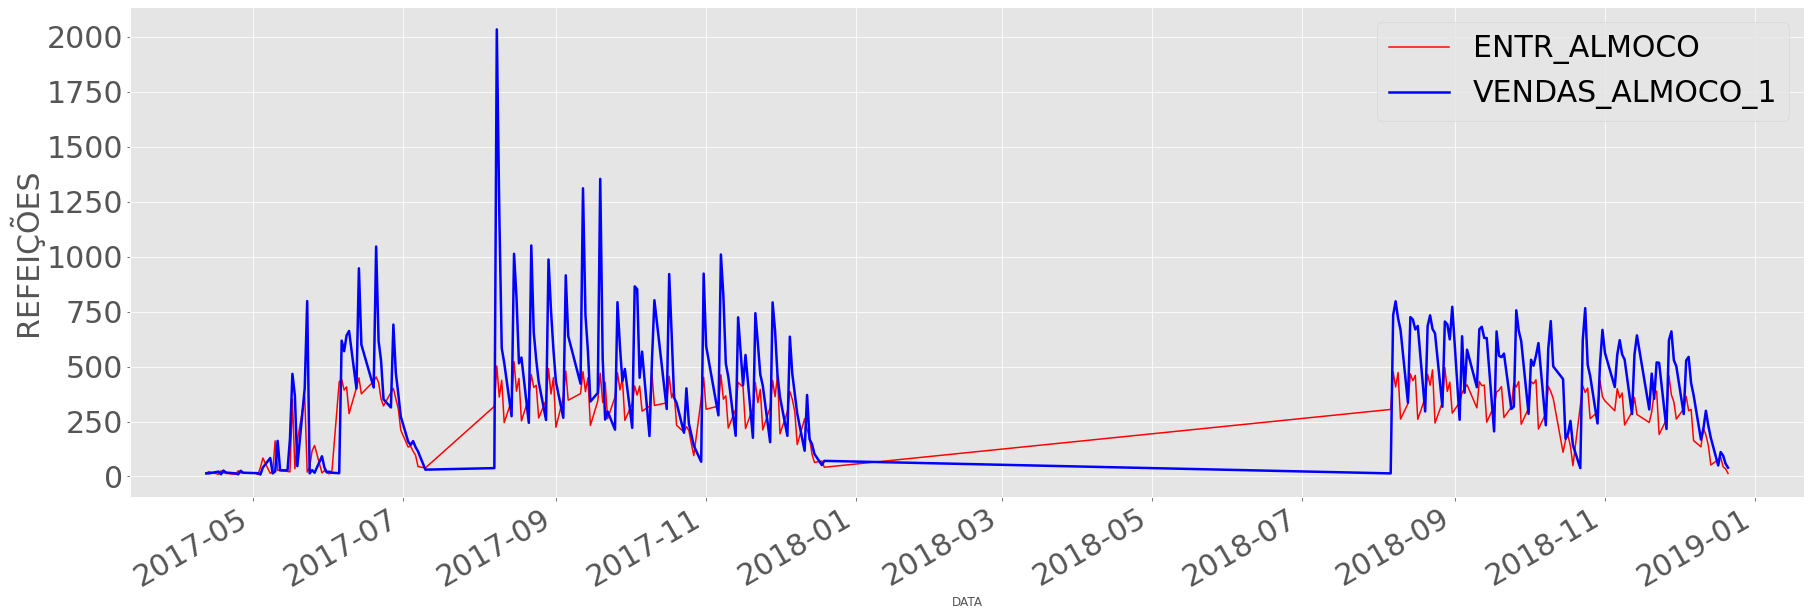
\includegraphics[width=1.0\textwidth]{./Figuras/resultados/case1_consumo_vendas_almoco.png}
                    	\caption{Correlação entre consumo e vendas de almoço.} \label{fig:case1_consumo_vendas_almoco} 
                    	}
                    \end{figure}
                \end{minipage} \hfill %
                \begin{minipage}[c]{0.3\textwidth}
                    \begin{figure}[H]
                    	\center{                    		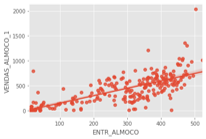
\includegraphics[width=1.0\textwidth]{./Figuras/resultados/case1_scatter_consumo_vendas_almoco.png}
                    	\caption{Gráfico Scatter entre consumo e vendas de almoço.} \label{fig:case1_scatter_consumo_vendas_almoco} }
                    \end{figure}
                \end{minipage} 
            \end{center}
            }
                
           \begin{table}[!ht]
           \centering
           \caption{Comparação de consumo com um dia anterior}
             \rowcolors{2}{gray!25}{white}
             \begin{tabular}{|c|c|}\hline
                \multicolumn{2}{c}{CONSUMO EM RELAÇÃO ÀS VENDAS DE 1 DIA ANTERIOR}\\ \hline
                CORRELAÇÃO (r) &  0.7255528038157009\\
                P-value &5.399561176138223e-41\\
                RMSE & 260.5399426736619\\
                TOTAL DE REFEIÇÕES PROJETADAS & 104694\\ 
                TOTAL DE REFEIÇÕES CONSUMIDAS & 69544\\
                TOTAL DE REFEIÇÕES SUB PROJETADAS & -4703\\
                TOTAL DE REFEIÇÕES SUPER PROJETADAS & 39853\\
                ERRO ABSOLUTO MEDIANO & 139.0\\
                ERRO ABSOLUTO PERCENTUAL MEDIO & 90.18\\\hline
            \end{tabular} \label{table:case1_vendas1} \end{table}

            \paragraph*{Normalização e escala de features}
                O processo de normalização e escala é demonstrado nesta seção com a feature de vendas de tickets de 1 dia anterior, pois entre todas as features esta é a que produziu outliers com maior destaque.
                A normalização dos dados é feita com o teto de 3x o desvio padrão médio, logo o pico de 2000 vendas foi normalizado para o valor arredondado de 1356 refeições e mesmo com a normalização, o comportamento linear desta feature, conforme figura \ref{fig:feature_sem_outliers}, se manteve.   
                E após a normalização foi realizada a aplicação da escala de 0 a 1 na feature e conforme é observado na figura  \ref{fig:feature_sem_outliers_escalada}, o comportamento linear da feature também se manteve.

                {
                    \begin{center}
                        \begin{minipage}[b]{1.0\textwidth}
                        \begin{figure}[H]
                        	\center{
                            	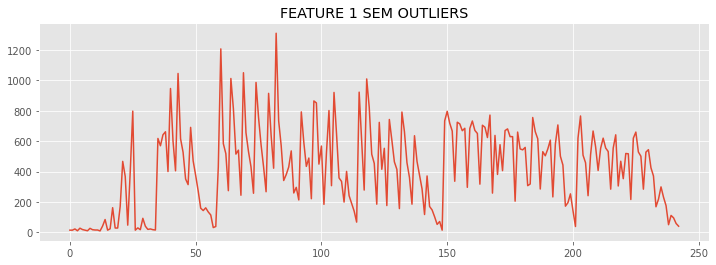
\includegraphics[width=1.0\textwidth]{./Figuras/resultados/feature_sem_outliers.png}
                            	\caption{Vendas de tickets normalizados com teto de 3x o desvio padrão.}
                            	\label{fig:feature_sem_outliers}
                        	}
                        \end{figure}
                        \end{minipage} \hfill %
                        
                        \begin{minipage}[b]{1.0\textwidth}
                        \begin{figure}[H]
                        	\center
                        	{                    		
                            	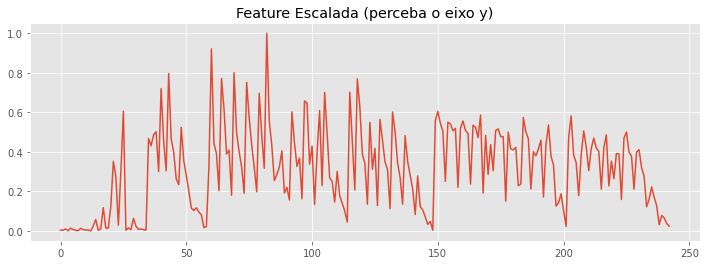
\includegraphics[width=1.0\textwidth]{./Figuras/resultados/feature_sem_outliers_escalada.png}
                            	\caption{Vendas de tickets escalada entre 0 a 1.} \label{fig:feature_sem_outliers_escalada} 
                        	}
                        \end{figure}
                        \end{minipage}
                    \end{center}
                }
                Este processo de normalização e escala foi realizado para todas as features endógenas e para as features climáticas.
        	   % \newpage
        	   
                \paragraph{Consumo atual em relação ao consumo do jantar de 1 dia anterior.}
                
                    Apesar de que os alunos que consomem refeições no almoço geralmente são de período e de grade horária diferente dos alunos que consomem o jantar no período da noite, nota-se uma relação evidente entre os 2 consumos, evidenciada pelo comportamento linear na figura \ref{fig:case1_consumo_jantar} com correlação (r) = 0.7655, e pela regressão linear entre esses 2 consumos na figura  \ref{fig:case1_consumo_jantar_scatter}, não foi possível encontrar uma causa evidente para este efeito anômalo.
                    
                    {\begin{center} 
                    \begin{minipage}[c]{1.0\textwidth}
                    \begin{figure}[H]
                    	\center{
                    	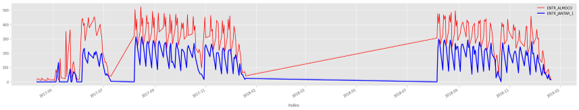
\includegraphics[width=1.0\textwidth]{./Figuras/resultados/case1_consumo_jantar.png}
                    	\caption{Correlação de consumo de almoço e jantar de 1 dia anterior.} 
                    	\label{fig:case1_consumo_jantar} }
                    \end{figure} 
                    \end{minipage}\hfill %
                    
                    \begin{minipage}[c]{0.3\textwidth}
                    \begin{figure}[H]
                    	\center{                    		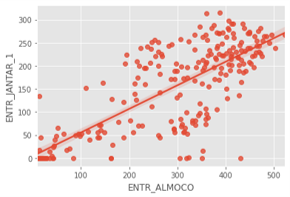
\includegraphics[width=1.0\textwidth]{./Figuras/resultados/case1_consumo_jantar_scatter.png}
                    	\caption{Gráfico Scatter entre consumo e jantar de 1 dia anterior.} 
                    	\label{fig:case1_consumo_jantar_scatter} }
                    \end{figure}
                    \end{minipage} \end{center} }
            
    	    \paragraph{Análise da sazonalidade semanal}
    	        Os gráficos de consumo a seguir da figura  \ref{fig:case1_violinplot_segunda}, representando a segunda-feira,  até a figura \ref{fig:case1_violinplot_sexta} , representando a sexta-feira,  são gerados para as features categóricas binárias, com a funcionalidade violin-plot da biblioteca seaborn, própria para distribuição de variáveis categóricas-binárias em um dataset.
    	        O violino azul com o valor 1 representa a distribuição do consumo ao longo do conjunto total de dados.
    	        O violino com valor zero pode ser ignorado e é um retorno padrão no gráfico da ferramenta, representando o complemento do consumo para o dia da semana considerado.
    	        Nas sextas feiras, o consumo teve escala de distribuição menor para todo o conjunto 2019. Foi notório que apesar da alternância de grades horárias durante a troca de semestres no ano de 2019, os dias de terça e quinta feira concentraram o maior movimento de consumo.
    	       %\newpage
    	       \begin{center}    
    	        \begin{minipage}[c]{0.45\textwidth}
    	         \begin{figure}[H]
                	\center{                		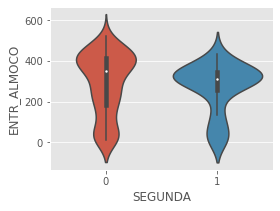
\includegraphics[width=\textwidth]{./Figuras/resultados/case1_segunda.png}
                	\caption{Gráfico violino da distribuição do consumo na segunda feira.} \label{fig:case1_violinplot_segunda} }
                \end{figure}\end{minipage} \hfill %
                      \begin{minipage}[c]{0.45\textwidth}
                \begin{figure}[H]
                	\center{                		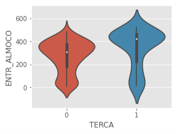
\includegraphics[width=\textwidth]{./Figuras/resultados/case1_terca.png}
                	\caption{Gráfico violino da distribuição do consumo na terça feira.} \label{fig:case1_violinplot_terca} }
                \end{figure} \end{minipage}
                 \begin{minipage}[c]{0.45\textwidth} 
                \begin{figure}[H]
                	\center{                		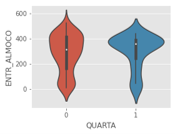
\includegraphics[width=\textwidth]{./Figuras/resultados/case1_quarta.png}
                	\caption{Gráfico violino da distribuição do consumo na quarta feira.	} \label{fig:case1_violinplot_quarta} }
                \end{figure}\end{minipage} \hfill %
                      \begin{minipage}[c]{0.45\textwidth}
                \begin{figure}[H]
                	\center{                		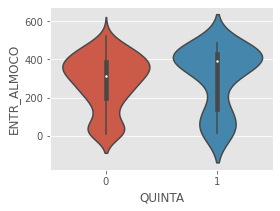
\includegraphics[width=\textwidth]{./Figuras/resultados/case1_quinta.png}
                	\caption{Gráfico violino da distribuição do consumo na quinta feira.} \label{fig:case1_violinplot_quinta} }
                \end{figure}\end{minipage} %
                        \begin{minipage}[c]{0.45\textwidth}
                \begin{figure}[H]
                	\center{                		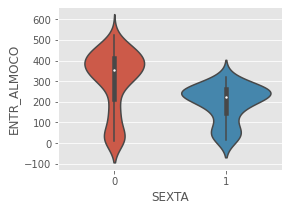
\includegraphics[width=\textwidth]{./Figuras/resultados/case1_sexta.png}
                	\caption{Gráfico violino da distribuição do consumo na sexta feira.} \label{fig:case1_violinplot_sexta} }
                \end{figure}
                \end{minipage} \end{center}
    \subsection{Análise das variáveis exógenas}
        As variáveis exógenas correspondem aos parâmetros, de domínio discreto, que são utilizados exclusivamente nos modelos de redes neurais mistos, e são lidos pelas camadas MLP destes modelos.
        \paragraph{Consumo atual em relação ao avanço do semestre}
        Para esta análise foi necessário restringir o domínio de análise para 1 semestre, o consumo em relação ao avanço do semestre teve queda abrupta nos ultimos dias do semestre, portanto a correlação dos conjuntos de dados das figuras \ref{fig:case1_perc_sem} e \ref{fig:case1_perc_sem_scatter} obteve valor negativo.
        {
        \begin{center} 
        
            \begin{minipage}[c]{1.0\textwidth}
                \begin{figure}[H]
                	\center{                    		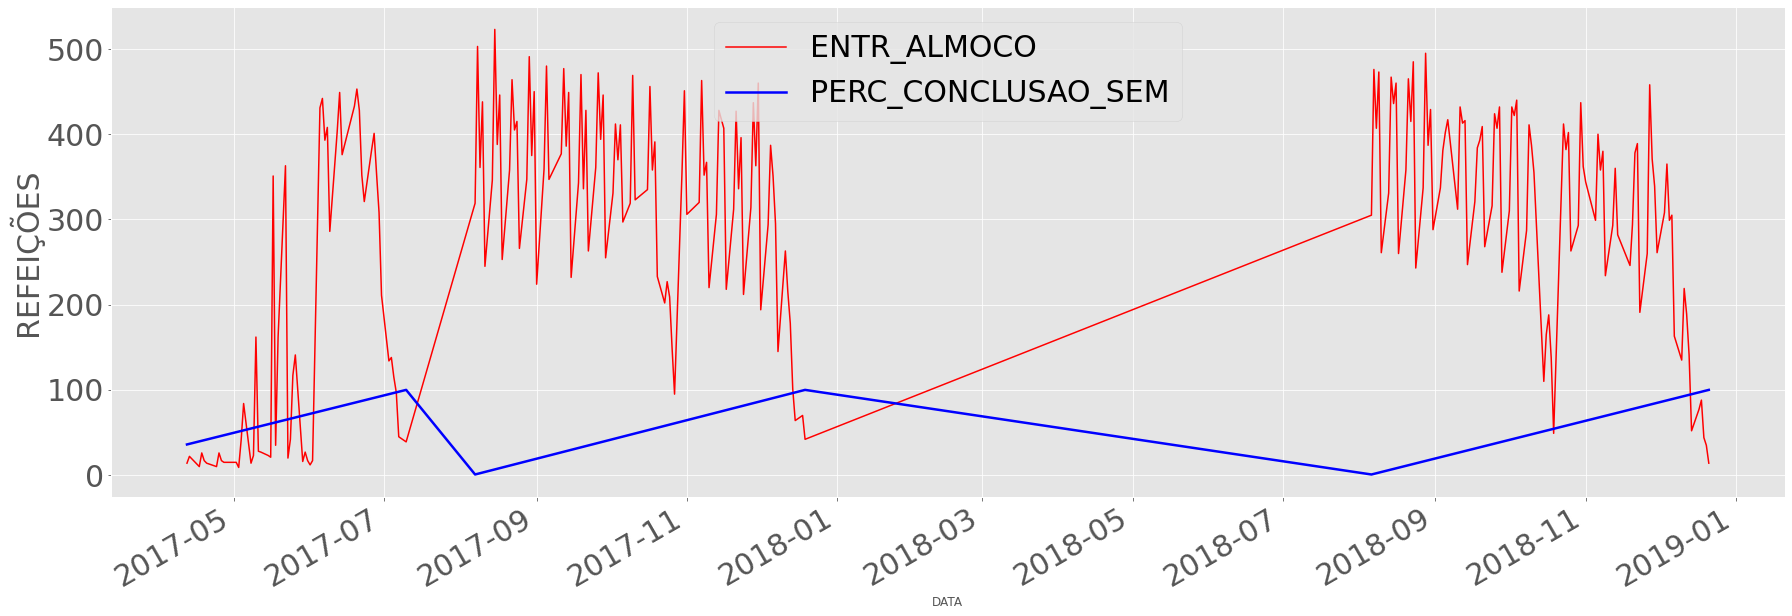
\includegraphics[width=\textwidth]{./Figuras/resultados/case1_perc_sem.png}
                	\caption{1a Fase : Relação da distribuição do consumo com o avanço do semestre, Correlação (r) = -0.35}
                	\label{fig:case1_perc_sem}
                	}
                \end{figure}  
            \end{minipage} \hfill %
        
            \begin{minipage}[c]{0.5\textwidth}
                \begin{figure}[H]
                	\center{                		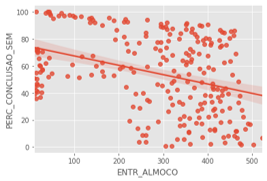
\includegraphics[width=\textwidth]{./Figuras/resultados/case1_perc_sem_scatter.png}
                	\caption{Gráfico scatter da distribuição do consumo com o avanço do semestre.} \label{fig:case1_perc_sem_scatter}
                	}
                \end{figure}
            \end{minipage} 
        \end{center} 
        }

\section{Protocolo Experimental}
\TODO{faça um resumo sobre as duas fases e as principais diferenças entre elas. Na sequência, detalhe os detalhes do principal modelo obtido (o com melhor resultado de predição)}
    
    \subsection{Avaliação do aprendizado do problema da predição de refeições por meio de redes neurais MLP}
        \paragraph{Ajuste empírico de topologia do primeiro modelo perceptron}
        O primeiro experimento com redes neurais realizado na primeira fase experimental, avaliou a capacidade de aprendizado do modelo perceptron sobre a sazonalidade dos dados endógenos, referentes ao domínio de consumo de refeições no R.U, verificando se o comportamento de consumo no restaurante pôde ser aprendido por este tipo de rede neural, portanto foi definida 1 rede neural inicial perceptron com apenas 1 camada oculta contendo 1 neurônio para 15 parâmetros de entrada (mesmo número de parâmetros endógenos) e com 1 neurônio de saída, denominada de MLP1.
        
        Os parâmetros endógenos correspondem à uma série temporal de intervalo de 5 dias anteriores para consumo de refeições no período do almoço, jantar e de vendas de tickets no período do almoço.
        O modelo foi denominado MLP1, sua ilustração pode ser visualizada na figura \ref{fig:case1_mlp1} obtida através da ferramenta NETRON. Cada camada do modelo MLP1 corresponde à um bloco com título \textbf{Dense} nesta figura, a primeira aresta da figura entre o bloco input e InputLayer demonstra as 3 séries temporais dos parâmetros de entrada, com intervalo de 5 dias passados cada. \textbf{ENTR\_ALMOCO, ENTR\_JANTAR e VENDAS\_ALMOCO}. O bloco Flatten converte cada dia de entrada das séries temporais em um parâmetro de entrada da rede neural MLP, conforme modelo conceitual do trabalho de \citeonline{Lopes2008} ilustrado na figura \ref{fig:mlp-lopes} que utiliza apenas 1 parâmetro endógeno com intervalo temporal também de 5 dias. A primeira camada oculta desta rede pode ser visualizada no primeiro bloco dense da figura que demonstra a função de ativação ReLu deste neurônio, e o número de unidades desta camada sendo 1.
        A camada de saída é o último bloco da figura, também com 1 unidade, e como a função de ativação é linear, ela não é exibida na descrição do bloco.
        \begin{figure}[H]
        \center{
        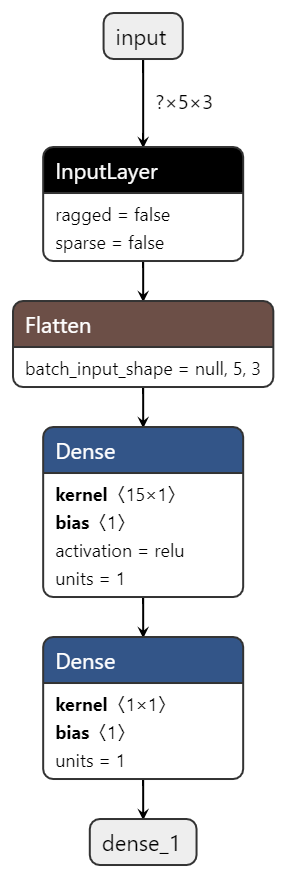
\includegraphics[width=0.3\textwidth]{./Figuras/resultados/case1_MLP1_validated.png}
        	\caption{Topologia do modelo MLP1, Ferramenta NETRON} 
        	\label{fig:case1_mlp1}
        }
        \end{figure}
        O treino deste modelo foi executado, obtendo RMSE com o valor 130,62 sobre o conjunto de validação, neste caso da primeira fase sendo os dados do primeiro semestre de 2018, e é possível notar figura \ref{fig:case1_mlp1_train} que as linhas da função de perda e treino convergiram à um processo de overfitting e não demonstraram aprendizado significante deste modelo sobre o conjunto de validação.
        \begin{figure}[H]
        	\center{
        	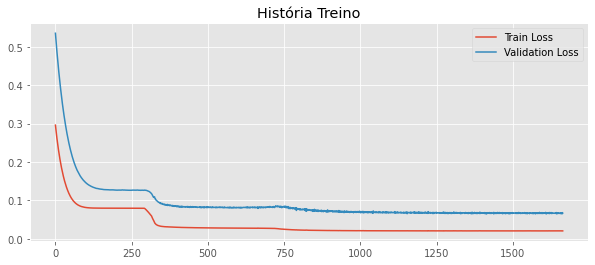
\includegraphics[width=0.8\textwidth]{./Figuras/resultados/case1_mlp1_train.png}
        	\caption{Gráfico de treino do modelo MLP1, RMSE = 130,62}
        	\label{fig:case1_mlp1_train}
        	}
        \end{figure}
        
        Portanto foi aumentada a profundidade do modelo MLP1 obtendo-se o modelo MLP2 com topologia ilustrada na figura  \ref{fig:case1_mlp2}, e após o treino deste modelo foi possível notar a diminuição do RMSE (Raiz do erro quadrático médio) para o valor de 107.97, observado na figura \ref{fig:case1_mlp2_train}. Validando a hipótese de que a predição do consumo no restaurante, pode ser aprendida por modelos simples de redes neurais, e portanto a pesquisa seguiu com a definição de novos modelos demonstrados na próxima subseção.
        \begin{figure}[H]
        	\center{
        		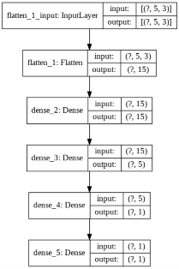
\includegraphics[width=0.3\textwidth]{./Figuras/resultados/case1_mlp2.png}
        	\caption{Topologia do modelo MLP2} \label{fig:case1_mlp2} }
        \end{figure}
        \begin{figure}[H]
        	\center{
        		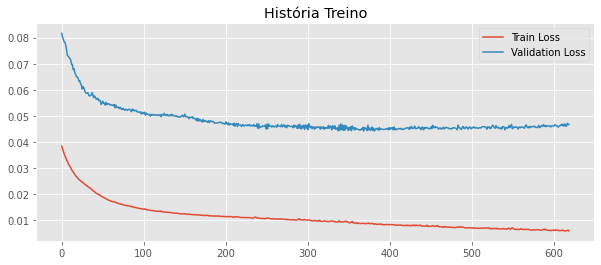
\includegraphics[width=1.0\textwidth]{./Figuras/resultados/case1_mlp2_train.png}
        	\caption{Gráfico de treino do modelo MLP2. RMSE = 107.97}
        	\label{fig:case1_mlp2_train} }
        \end{figure}
    \subsection{Definições das topologias dos modelos}
        \paragraph{Modelo endógeno MLP\_ENDO\_1}
            O primeiro modelo experimental MLP para obtenção das predições tem topologia definida na figura \ref{fig:case1_mlp_endo1}, denominado MLP\_ENDO\_1, este modelo tem 64 neurônios na primeira camada oculta e 32 neurônios na segunda camada oculta, e assim como todos os outros modelos, 1 neurônio na camada de saída. Ressaltando que a metodologia do cap \ref{cap:metodos} define que para os modelos MLP as camadas ocultas utilizam função de ativação ReLu e função de saída Linear.
            \begin{figure}[H]
            	\center{                		
            	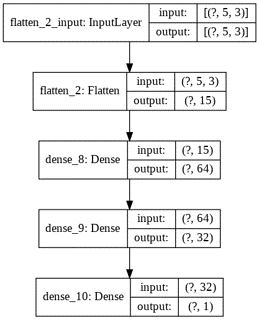
\includegraphics[width=0.25\textwidth]{./Figuras/resultados/case1_mlp_endo1.png}
            	\caption{Topologia do modelo MLP\_ENDO\_1} 
            	\label{fig:case1_mlp_endo1} 
            	}
            \end{figure}
            
         \paragraph{Modelo endógeno GRU RNN\_ENDO\_1}
            Este primeiro modelo experimental GRU foi definido com 16 unidades GRU, com topologia conceitual definida de acordo com a figura \ref{fig:gru-arch} no capítulo de fundamentação teórica \textbf{MLP\_ENDO\_1} e tem um neurônio perpcetron para emissão do sinal de saída, representado pelo bloco\textbf{Dense} na figura \ref{fig:case1_rnn_endo1}
            \begin{figure}[H]
              \center{
                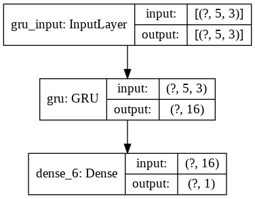
\includegraphics[width=0.25\textwidth]{./Figuras/resultados/case1_rnn_endo1.png}
                \caption{Topologia do modelo RNN\_ENDO\_1} \label{fig:case1_rnn_endo1} }
            \end{figure}
         
         \paragraph{Modelo endógeno GRU RNN\_ENDO\_2}
           Foi definido uma segunda reconfiguração do modelo GRU, RNN\_ENDO\_2, com o aumento da profundidade de unidades do modelo anterior RNN\_ENDO\_1, em formato regressivo de 16 unidades na primeira camada, 8 unidades na segunda e 4 na terceira, e com a inclusão do recurso Dropout entre as unidades para eliminar unidades com pesos negativos no grafo denso da rede, observado na figura \ref{fig:case1_rnn_endo2} realizando a poda de unidades não relevantes durante o treino.
            \begin{figure}[H]
              \center{
                  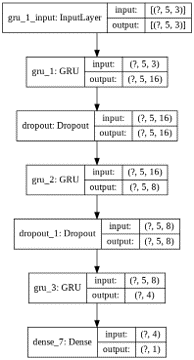
\includegraphics[width=0.20\textwidth]{./Figuras/resultados/case1_rnn_endo2.png}
                  \caption{Topologia do modelo RNN\_ENDO\_2} 
                  \label{fig:case1_rnn_endo2} 
              }
            \end{figure}
        \paragraph{Modelo misto RNN\_EXO\_1}
            Interpretando o digrama do primeiro modelo misto,  \textbf{RNN\_EXO\_1}, na figura \ref{fig:case1_rnn_exo_1}o bloco com título GRU à esquerda na figura de topologia do modelo, trata as entradas endógenas (temporais), assim como exemplificado nos modelos GRU endógenos. O bloco com título \textbf{Dense} é uma rede MLP que recebe um input com 10 parâmetros de 1 dimensão, portanto todos discretos, correspondendo aos 4 parâmetros climáticos (temperatura, umidade, pressão e vento), 1 parâmetro para o dia da semana vigente, 1 para o semestre vigente e 4 parâmetros de controle do calendário (distancia da data anterior, posterior, avanço do semestre, avanço do mês). A saída dos blocos GRU e MLP são concatenadas e tratadas pelo bloco MLP de saída.
            \begin{figure}[H]
              \center{
                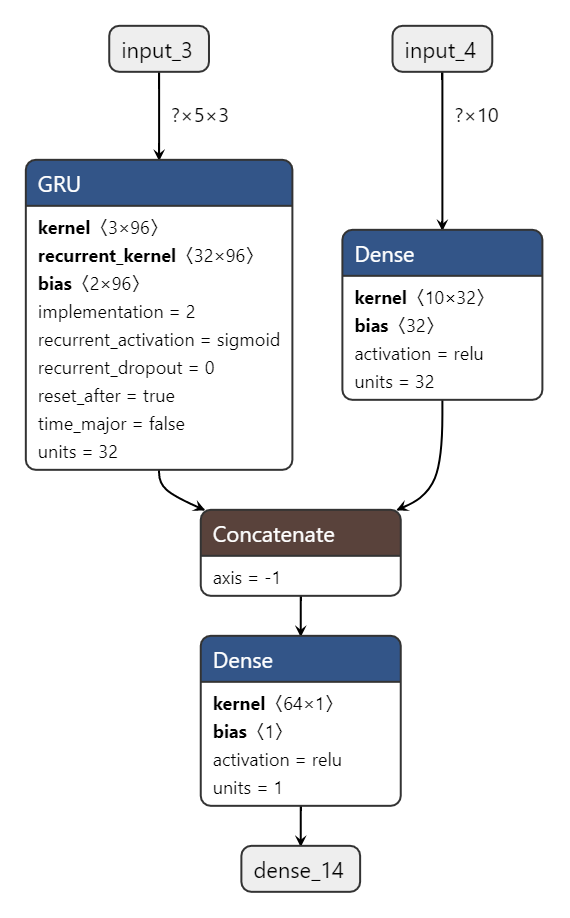
\includegraphics[width=0.7\textwidth]{./Figuras/resultados/case1_rnn_exo_1.png}
                \caption{Topologia do modelo RNN\_EXO\_1} \label{fig:case1_rnn_exo_1} }
            \end{figure}
            
        \paragraph{Modelo misto RNN\_EXO\_2}
         O Segundo modelo misto foi definido com o aumento da profundidade das camadas GRU e MLP do modelo anterior, conforme observado na figura \ref{fig:case1_rnn_exo_2} foram acrescentadas 1 camada GRU e 1 camada MLP (Dense).
            \begin{figure}[H]
              \center{
                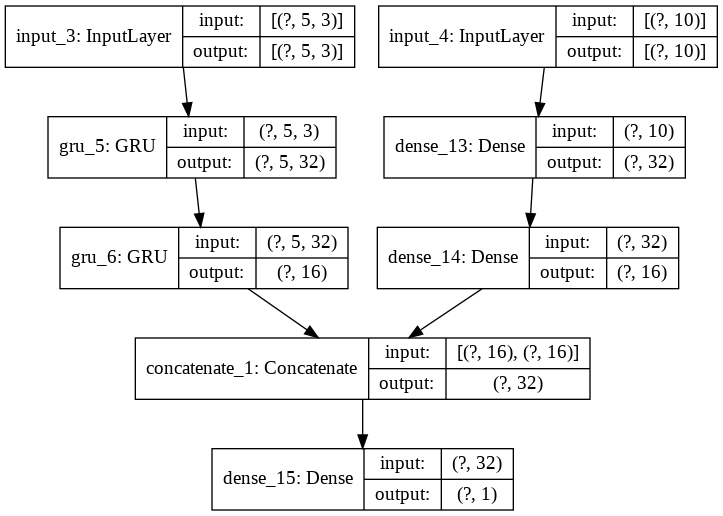
\includegraphics[width=0.6\textwidth]{./Figuras/resultados/case1_rnn_exo_2.png}
              \caption{Topologia do modelo RNN\_EXO\_2}  \label{fig:case1_rnn_exo_2} }
            \end{figure}
        
        \paragraph{Modelo misto RNN\_EXO\_3}
        Para o terceiro e último modelo misto, representado na figura \ref{fig:case1_rnn_exo_3}, foi feita uma reconfiguração do modelo misto anterior com a utilização do recurso dropout nas saídas das camadas GRU, que realiza podas de conexões com pesos negativos.
        \begin{figure}[H]
          \center{
          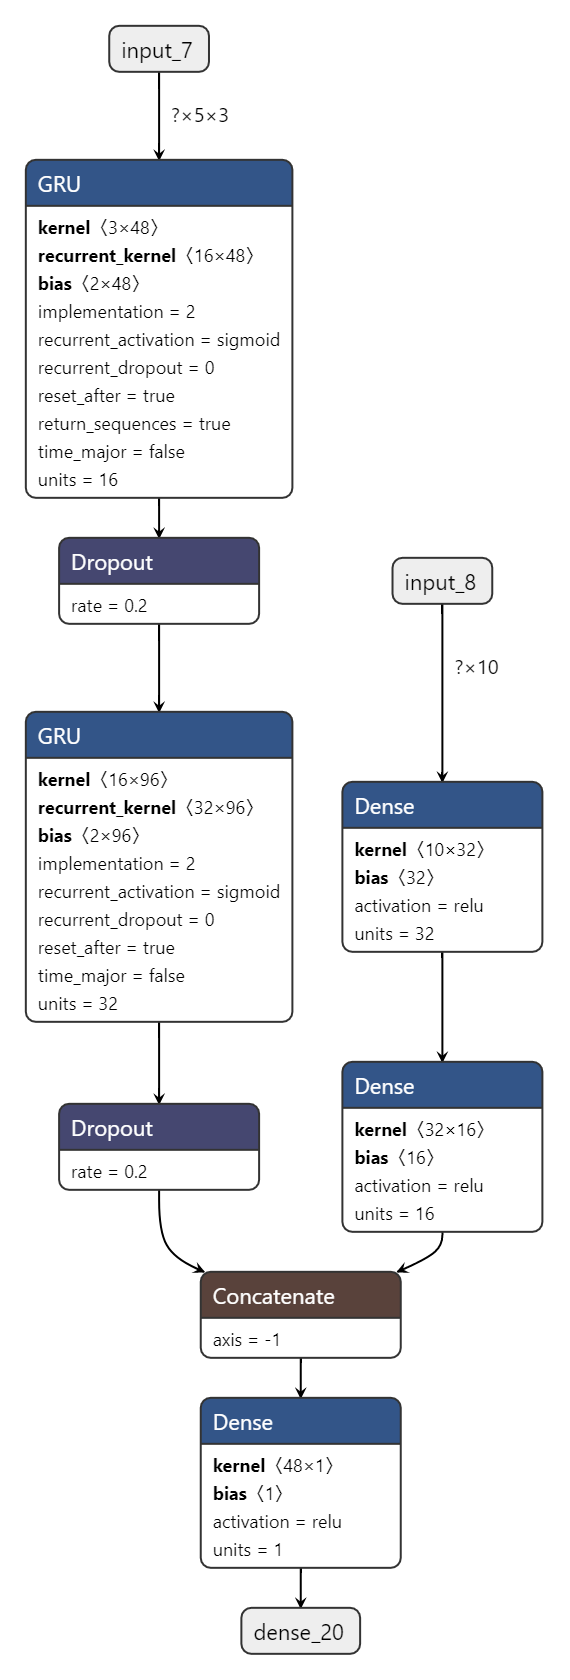
\includegraphics[width=0.5\textwidth]{./Figuras/resultados/case1_rnn_exo_3.png}
          \caption{Topologia do modelo RNN\_EXO\_3} \label{fig:case1_rnn_exo_3} 
          }
        \end{figure}
    \subsection{Diferenças principais dos resultados entre as fases experimentais}
        \paragraph{Diferenças entre os melhores modelos}
        Para os experimentos da 1a fase, o modelo que produziu o menor RMSE no conjunto de testes com vantagem em todas as outras métricas foi o modelo endógeno, RNN\_ENDO\_2, com algumas anomalias de predição observadas na figura \ref{fig:case1_rnn_endo2_test_dates}.
        \begin{figure}[H]
          \center{
            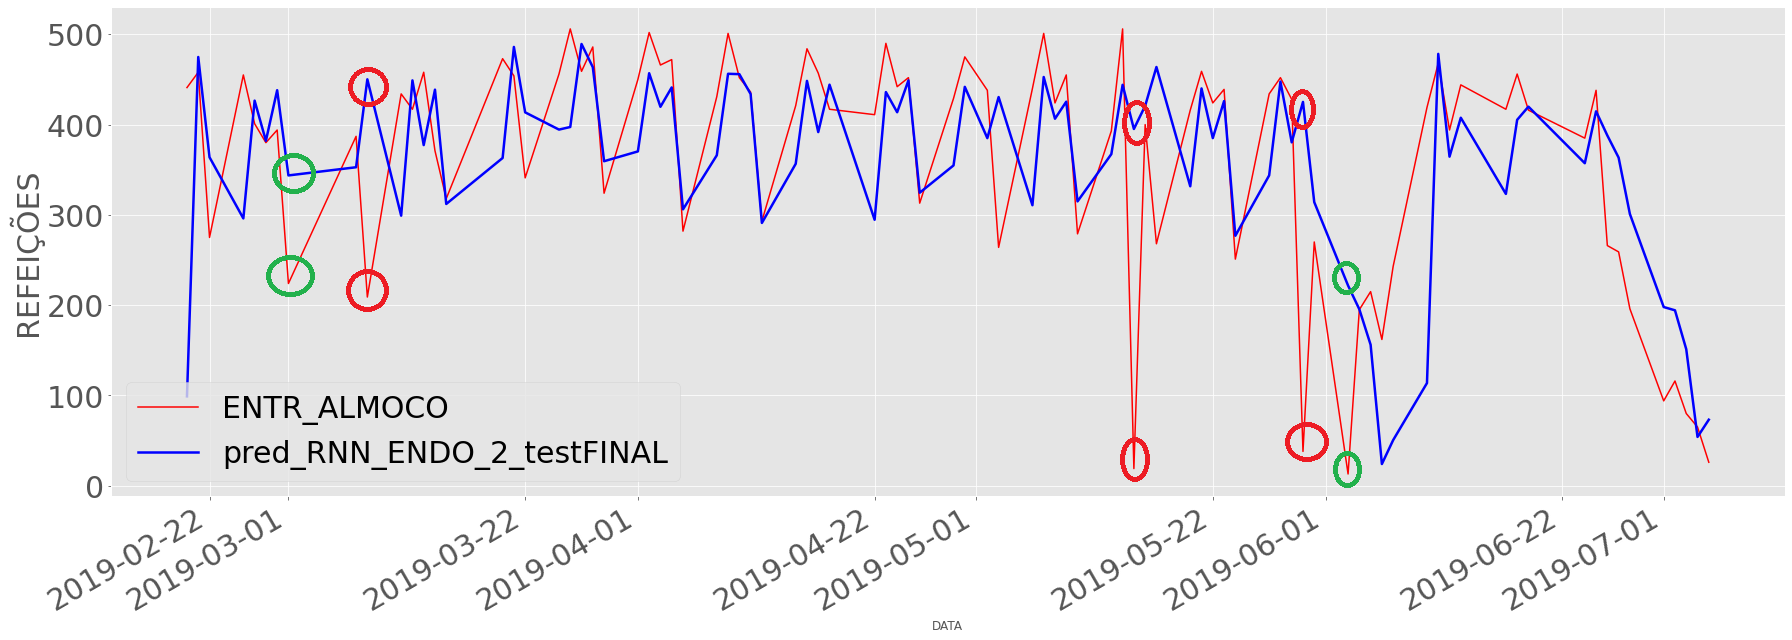
\includegraphics[width=1.0\textwidth]{./Figuras/resultados/case1_rnn_endo2_test_dates.png}
          \caption{Analise de anomalias preditivas do RNN\_ENDO\_2} \label{fig:case1_rnn_endo2_test_dates} }
        \end{figure}
        
        Os pontos verdes outliers representam predições que corresponderam a tendência de alta ou baixa de consumo mas com erros discrepante, e os pontos vermelhos representam predições com tendência inversa ao consumo.
        As justificativas para a predição dentro da tendência, se encontram na tabela \ref{table:rnn_endo_2_green}, denotando datas especiais que não poderiam corresponder ao processo de aprendizado do modelo.
            \begin{table}[!ht]
                \centering
                \caption{Erros de predições do modelo RNN\_ENDO\_2 na 1a fase}
                \label{table:rnn_endo_2_green}
                \rowcolors{2}{gray!25}{white}
                 \begin{tabular}{|c|c|c|}
                 \rowcolor{gray!50}
                 \hline 
                Data & Consumo & Justificativa\\ \hline    
                01/03/2019 (sexta feira)    & 224 & Sexta Feira pré - carnaval\\
                03/06/2019 (segunda feira)  &  13 & Segunda Feira pós paralisação estudantil\\ \hline 
                \end{tabular} 
            \end{table}
            
        As justificativas para previsões onde o modelo seguiu tendência oposta ao consumo também corresponderam à datas especiais, conferidas na tabela \ref{table:rnn_endo_2_red}.
            \begin{table}[!ht]
                \caption{Anomalias de predições do modelo RNN\_ENDO\_2 na 1a fase}
                \label{table:rnn_endo_2_red}
                \rowcolors{2}{gray!25}{white}
                 \begin{tabular}{|c|c|c|}
                 \rowcolor{gray!50}
                 \hline
                Data & Consumo & Justificativa \\
                08/03/2019 (sexta feira)   & 209 &Sexta Feira pós - carnaval\\
                15/05/2019 (quarta feira)   & 19  & Paralisação estudantil na praça Afonso Pena\\
                30/05/2019 (quinta feira)   &  38  & Paralisação estudantil na Praça Afonso pena\\
                \hline 
                \end{tabular} 
            \end{table}
        
        Nas métricas deste modelo, é observado na tabela \ref{table:rnn_endo_2_test} que a soma dos erros positivos, correspondeu à um descarte de aproximadamente 3479 refeiçoes, e o erro quadrático médio de previsão foi de aproximadamente 108 refeições.
            \begin{table}[!ht]
                \centering
                \rowcolors{2}{gray!25}{white}
                \caption{Métricas do melhor modelo:  RNN\_ENDO\_2 }
                \label{table:rnn_endo_2_test}
                \begin{tabular}{|c|c|}
                \rowcolor{gray!50}
                \hline
                Melhor modelo: &   RNN\_ENDO\_2: \\ \hline
                Total\_Consumidas & 31962 \\ 
                Total\_Previstas & 31465,61133 \\
                Erro\_Total\_Previsao & -496,3886719 \\
                Percentual\_Erro\_Total & -1,5530\% \\\
                Correlação & 0,595439895 \\
                P-value & 9,42215E-10    \\
                RMSE &  108,0663015\\
                Soma dos erros Negativos & -2982,567947 \\
                Soma dos erros Positivos & 3478,957266\\
                ERRO\_ABS\_MEDIANO & 46,70721436 \\ 
                ERRO\_ABSOLUTO\_PERCENTUAL\_MEDIO & 74,93539002 \\ 
                \hline
                \end{tabular}
            \end{table}
        
        Já na segunda fase, todos os modelos obtiveram melhoras no erro de treino sobre o conjunto de validação, e foi obtido o modelo com as melhores predições do trabalho, o modelo misto \textbf{RNN\_EXO\_1} detalhado em sua própria seção a seguir.
        É importante notar que as 2 fases produziram melhores modelos de classes distintas, a primeira com um modelo que utiliza apenas dados endógenos, e que contempla um conjunto de validação e teste com amplitude de apenas 1 semestre, e a segunda com um modelo que utiliza dados temporais e discretos, e que utiliza conjunto de validação e teste com amplitude de 1 ano.
        Isso denota que resultados melhores foram conquistados sem nenhuma alteração de parâmetros e hiper-parâmetros nos modelos, alterando-se apenas a organização temporal dos conjuntos de dados.
        
        Durante o teste de todos os modelos, apenas o primeiro semestre contemplou datas especiais onde estes modelos produziram anomalias de previsões, ilustrado como exemplo na figura \ref{fig:case1_rnn_endo2_test_dates}.

\section{Resultados com o Modelo RNN\_EXO\_1}
\TODO{Nessa seção apresente os resultados do melhor modelo. Se quiser, pode dividir em subseções}
    Este modelo, representado na figura \ref{fig:case1_rnn_exo_1} obteve os melhores resultados de todo este trabalho quando foi treinando na segunda fase experimental.
    É notório sua melhoria de resultados com uma única mudança da organização dos conjuntos de dados entre as fases experimentais.
    
    \subsection{Comparativo do treino entre as duas fases}
     Nota-se que este modelo produziu um gráfico função de perda durante o treino, com comportamento oscilatório pior, convergindo mais rapidamente à um overfitting, na primeira fase, ilustrado na figura \ref{fig:case1_rnn_exo_1_train} em comparação ao treino com melhores resultados na segunda fase, ilustrado na figura \ref{fig:case2_rnn_exo1_train}. É notório também a diferença das métricas RMSE entre estes 2 treinos, produzindo um resultado melhor na segunda fase, de RMSE = 109,97 em comparação ao resultado da primeira fase de RMSE = 132,94.
     
     \paragraph{Resultados de treino e validação para a primeira fase}
     {
        \begin{center} \begin{minipage}[c]{1.0\textwidth}
        \begin{figure}[H]
        \center{                    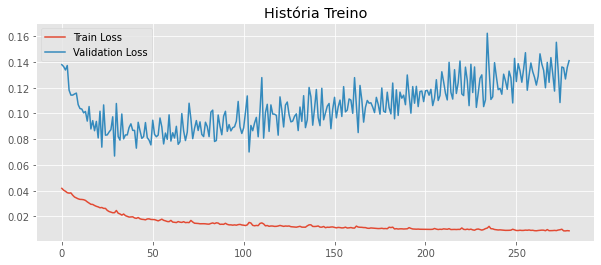
\includegraphics[width=\textwidth]{./Figuras/resultados/case1_rnn_exo_1_train.png}
        \caption{Treino do modelo RNN\_EXO\_1 na 1a fase, RMSE = 132.94} \label{fig:case1_rnn_exo_1_train} }
        \end{figure}
        \end{minipage} \hfill %
        \end{center} 
      }
     
    \paragraph{Resultados de treino e validação para a segunda fase}
    {\begin{center} \begin{minipage}[b]{1.0\textwidth}
        \begin{figure}[H]
          \center{
            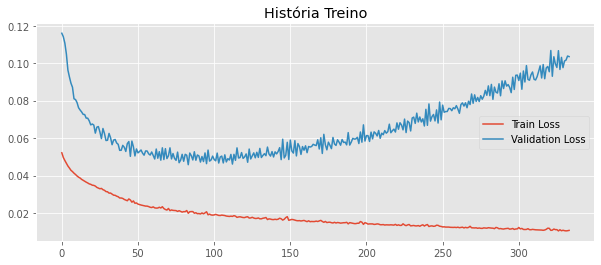
\includegraphics[width=\textwidth]{./Figuras/resultados/case2/case2_rnn_exo1_train.png}
          \caption{Gráfico de treino do modelo RNN\_EXO\_1 na 2a fase, RMSE = 109.97} \label{fig:case2_rnn_exo1_train} }
        \end{figure}\end{minipage} \hfill %
        \end{center} }
    
    \subsection{Comparativo de teste do modelo no primeiro semestre, entre as 2 fases}
        Como este modelo treinado na segunda fase obteve os melhores resultados do trabalho, foram recalculadas as métricas para o teste de modelo dentro do domínio do primeiro semestre de 2019 para realizar uma comparação justa com sua versão treinada e testada também no primeiro semestre de 2019 na primeira fase.
        
        A tabela \ref{table:case1_rnn_exo_1} demonstra que o RMSE de teste do modelo treinado na primeira fase foi notoriamente maior, e portanto pior, do que o RMSE treinado na segunda fase de acordo com a tabela \ref{table:case2_rnn_exo_2_incase1}. O RMSE sendo menor no treino deste modelo na segunda fase já trás uma melhoria em todas as outras métricas em comparação com o seu treino na primeira fase.
        A soma dos erros positivos de predições também foi menor na segunda fase, o que impacta menor em descarte de refeições.
        O RMSE deste modelo testado na primeira fase e alcançando RMSE = 106,2080 também se saiu melhor do que o melhor modelo da primeira fase, o RNN\_ENDO\_2 que alcançou RMSE = 108,06.
        
        O gráfico scatter do modelo treinado na primeira fase, conforme figura \ref{fig:case1_rnn_exo_1_test_scatter} também se saiu pior, mais distante da borda superior direita do gráfico, em relação ao scatter do modelo treinado na segunda fase conforme a figura \ref{fig:case2_rnn_exo2_test_incase1_scatter}.
        
        Por fim na comparativa entre os gráficos de predição, o modelo RNN\_EXO\_1 treinado na primeira fase produziu predições piores, e não aprendeu a sazonalidade semanal do consumo, como pode ser observado na figura \ref{fig:case1_rnn_exo_1_test}, é possível notar também, na tabela  \ref{table:case1_rnn_exo_1}, que a correlação entre os valores previstos e o consumo real, bem como o valor $R^2$ foi inferior em comparação às métricas do modelo treinado na segunda fase, e que este modelo treinado na segunda fase aprendeu melhor a sazonalidade semanal e mensal do consumo como pode ser observado na figura \ref{fig:case2_rnn_exo2_test_incase1}.
        
        \paragraph{Teste para o 1o semestre, treino na 1a fase}
            {
    	    \begin{center} 
    	        \begin{minipage}[c]{1.0\textwidth}
                  \begin{figure}[H]
                      \center{                    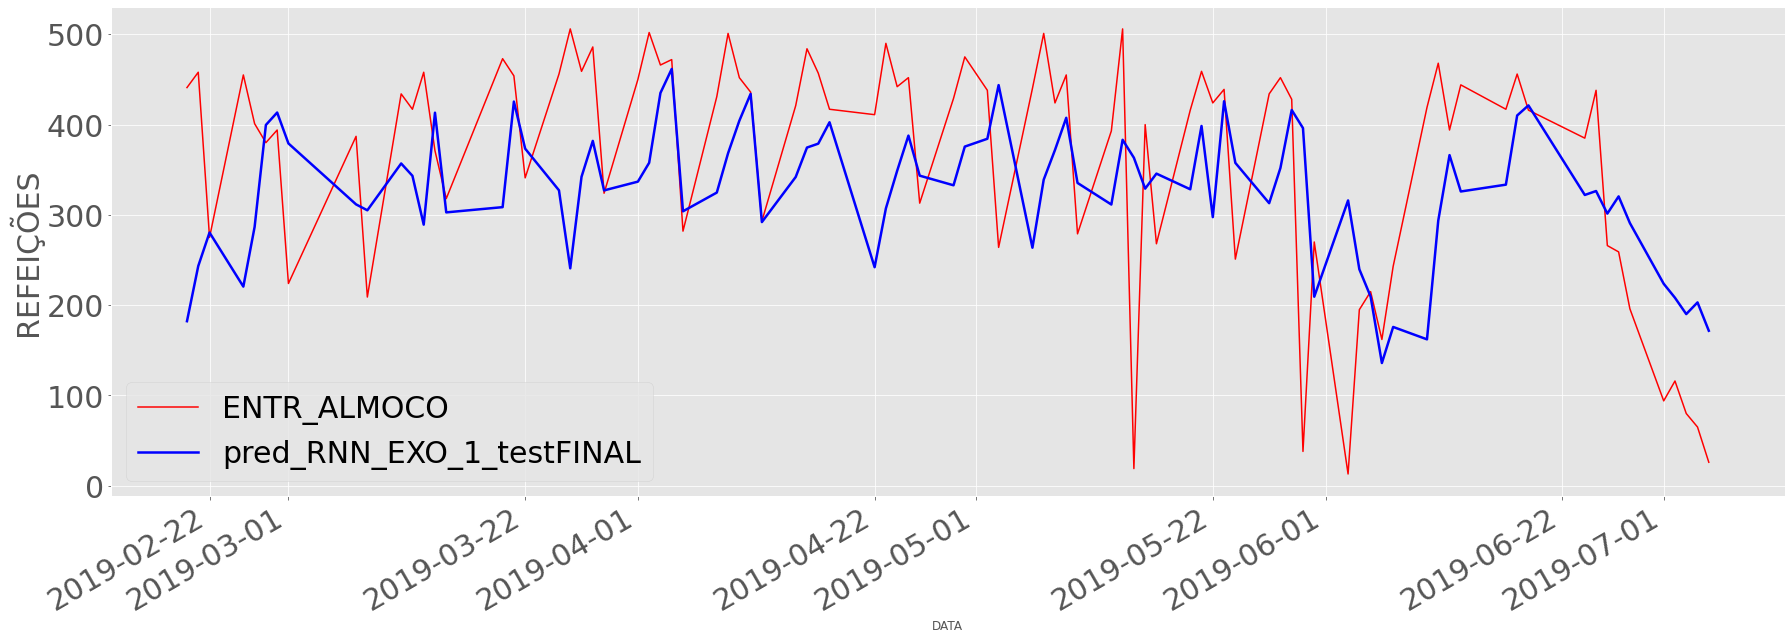
\includegraphics[width=\textwidth]{./Figuras/resultados/case1_rnn_exo_1_test.png}
                      \caption{Teste do modelo RNN\_EXO\_1, 1a fase} 
                      \label{fig:case1_rnn_exo_1_test} }
                    \end{figure} 
                \end{minipage} \hfill %
                
                \begin{minipage}[c]{0.5\textwidth}
                    \begin{figure}[H]
                      \center{                    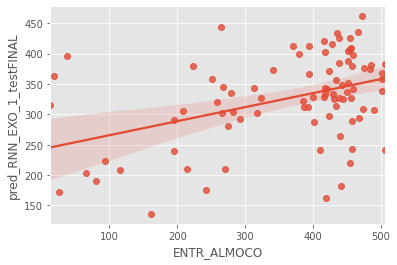
\includegraphics[width=\textwidth]{./Figuras/resultados/case1_rnn_exo_1_test_scatter.png}
                        \caption{Gráfico scatter de teste do modelo RNN\_EXO\_1, 1a fase} \label{fig:case1_rnn_exo_1_test_scatter} }
                        \end{figure}
                \end{minipage} 
            \end{center} }
            
            \begin{table}[!ht]
            \centering
            \caption{RNN\_EXO\_1 TREINADO NA 1A FASE,TESTE 1o SEMESTRE 2019}
            \label{table:case1_rnn_exo_1}
            \rowcolors{2}{gray!25}{white}
                \begin{tabular}{|c|c|}
                \rowcolor{gray!50}
                \hline
            \multicolumn{2}{c}{RNN\_EXO\_1 TREINADO NA 1A FASE,TESTE 1o SEMESTRE 2019} \\
            \hline
            RMSE & 124.49\\
            TOTAL DE REFEIÇÕES CONSUMIDAS & 31962 \\
            TOTAL DE REFEIÇÕES PROJETADAS & 28728.816  \\
            ERRO DE PREVISÃO & -3233.1839375 \\
            PERCENTAGEM DE ERRO & -10.11\%  \\
            CORRELAÇÃO (r) & 0.41 \\ 
            P-value & 6.59e-05\\ 
            R2 & 0.16\\
            SOMA DOS ERROS NEGATIVOS & -2709.17\\
            SOMA DOS ERROS POSITIVOS & 5942.35\\
            ERRO ABSOLUTO MEDIANO & 85.59\\
            ERRO ABSOLUTO PERCENTUAL MÉDIO & 90.98\% \\ \hline \end{tabular} \end{table}
        
        \paragraph{Teste para o 1o semestre, treino na 2a fase}
            \begin{table}[!ht]
            \centering
            \caption{RNN\_EXO\_1 TREINADO NA 2A FASE, TESTE 1o SEMESTRE 2019}
            \label{table:case2_rnn_exo_2_incase1}
            \rowcolors{2}{gray!25}{white}
                \begin{tabular}{|c|c|}
                \rowcolor{gray!50}
                \hline
                \multicolumn{2}{c}{RNN\_EXO\_1 TREINADO NA 2A FASE, TESTE 1o SEMESTRE 2019}\\ \hline
                RMSE & 106.2080\\
                TOTAL DE REFEIÇÕES CONSUMIDAS & 31962\\
                TOTAL DE REFEIÇÕES PROJETADAS & 32170.24\\
                ERRO DE PREVISÃO & 208.2460 \\
                PERCENTAGEM DE ERRO & 0.6515\%  \\
                CORRELAÇÃO (r)& 0.5903766574738285 \\
                P-value (p) & 1.4143e-09\\
                R2 & 0.3485\\
                SOMA DOS ERROS NEGATIVOS & -3454.8698\\
                SOMA DOS ERROS POSITIVOS & 3246.6228\\
                ERRO ABSOLUTO MEDIANO & 59.5414\\
                ERRO ABSOLUTO PERCENTUAL MÉDIO & 83.2671\% \\ \hline
            \end{tabular}
            \end{table}
            {
            \begin{center} 
            \begin{minipage}[c]{1.0\textwidth}
            \begin{figure}[H]
              \center{
                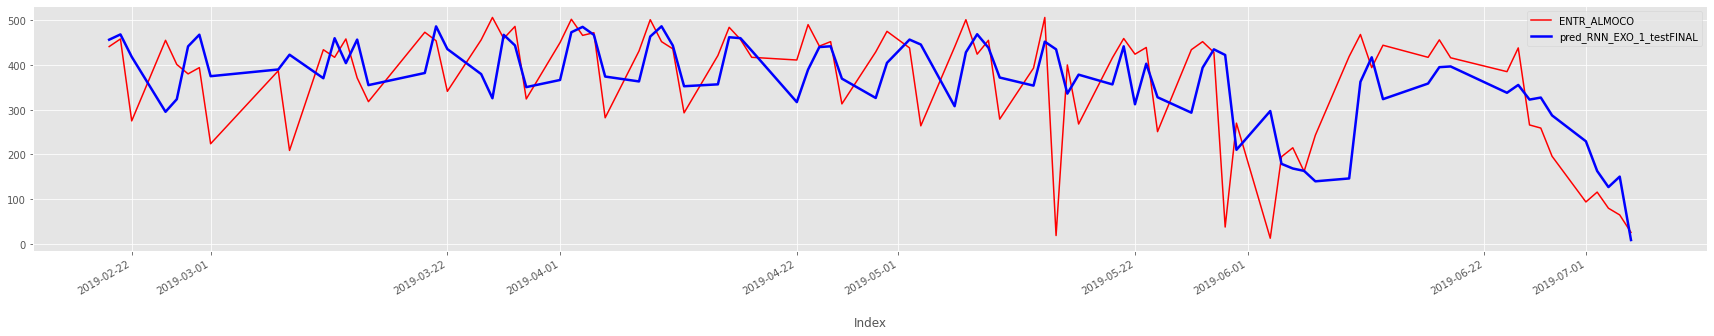
\includegraphics[width=\textwidth]{./Figuras/resultados/case2/case2_rnn_exo2_test_incase1.png}
              \caption{Gráfico teste do primeiro semestre do RNN\_EXO\_1 treinado na segunda fase} \label{fig:case2_rnn_exo2_test_incase1} }
            \end{figure}
            \end{minipage} \hfill %
            
            \begin{minipage}[c]{0.45\textwidth}
            \begin{figure}[H]
              \center{
                \includegraphics[width=\textwidth]{./Figuras/resultados/case2/case2_rnn_exo2_test_incase1_scatter.png}
              \caption{Gráfico scatter de teste do primeiro semestre, RNN\_EXO\_1 treinado na segunda fase} \label{fig:case2_rnn_exo2_test_incase1_scatter} }
                \end{figure}
                \end{minipage} 
                \end{center} 
            }
    \subsection{Teste final do modelo}
     O teste final do modelo RNN\_EXO\_1 por fim produziu os melhores resultados com seu treino na segunda fase e sendo testado para o ano inteiro de 2019. O RMSE observado na tabela \ref{table:case2_rnn_exo_2_2019} foi notoriamente inferior à todos os modelos treinados e testados em todo o trabalho.
     O descarte de refeições obtido pela soma dos erros positivos atingiu o valor de 4768 refeições.
     É possível notar na figura \ref{fig:case2_rnn_exo1_test} que o modelo aprendeu bem a sazonalidade mensal e semanal do consumo, mas obteve erro discrepante para o primeiro valor previsto do segundo semestre, o erro foi justificável pois seu conjunto de treino contempla apenas 1 ano com 1 alternância de semestre impossibilitando um aprendizado melhor sobre este comportamento.
     O gráfico scatter ilustrado na figura \ref{fig:case2_rnn_exo1_test_scatter} também demonstra uma boa regressão linear sobre os valores previstos pelo modelo e o valor real de consumo, se aproximando da função identidade de uma previsão ideal.
     
     {\begin{center} \begin{minipage}[c]{1.0\textwidth}
        %%% RNN_EXO_1
        \begin{figure}[H]
          \center{
            \includegraphics[width=\textwidth]{./Figuras/resultados/case2/case2_rnn_exo1_test.png}
          \caption{Gráfico final de teste do modelo RNN\_EXO\_1.} \label{fig:case2_rnn_exo1_test} }
        \end{figure}
        \end{minipage} \hfill %
         \begin{minipage}[c]{0.5\textwidth}
        \begin{figure}[H]
          \center{
            \includegraphics[width=\textwidth]{./Figuras/resultados/case2/case2_rnn_exo1_test_scatter.png}
          \caption{Gráfico de scatter do modelo  RNN\_EXO\_1.} \label{fig:case2_rnn_exo1_test_scatter} }
        \end{figure}
        \end{minipage} \end{center} }
        \begin{table}[!ht]
            \centering
            \caption{RNN\_EXO\_1 TREINADO NA 2A FASE, TESTE ANO DE 2019}
            \label{table:case2_rnn_exo_2_2019}
            \rowcolors{2}{gray!25}{white}
                \begin{tabular}{|c|c|}
                \rowcolor{gray!50}
                \hline
                \multicolumn{2}{c}{RNN\_EXO\_1 TREINADO NA 2A FASE, TESTE ANO DE 2019}\\ \hline
                RMSE & 99.36\\
                TOTAL DE REFEIÇÕES CONSUMIDAS & 58653 \\
                TOTAL DE REFEIÇÕES PROJETADAS & 62048.04\\
                ERRO DE PREVISÃO & 3395.04 \\
                PERCENTAGEM DE ERRO & 5.78\%  \\
                CORRELAÇÃO (r)& 0.67 \\
                P-value (p) & 3.29e-25\\
                R2 & 0.45\\
                SOMA DOS ERROS NEGATIVOS & -8163.18\\
                SOMA DOS ERROS POSITIVOS & 4768.13\\
                ERRO ABSOLUTO MEDIANO & 55.23\\
                ERRO ABSOLUTO PERCENTUAL MÉDIO & 83.2671\% \\ \hline
            \end{tabular}
            \end{table}



    \chapter{Conclusão} \label{cap:conclusoes}

    Primeiramente, neste trabalho foi possível avaliar importância da metodologia de divisão do conjunto de dados em séries temporais.Visto que com um conjunto de dados de sazonalidade temporal, é notório que a ordenação dos dados na separação dos conjuntos de treino, teste e validação devem seguir uma ordem cronológica para os modelos aprenderem com o passado e realizarem predições para o futuro. O comportamento anômalo da predição identificada no capitulo de divisão do conjunto de dados da fase 1, demonstrado na figura \ref{fig:pandas_wrong_indexing}, e sua eliminação após a organização correta da série temporal, conforme a figura \ref{fig:pandas_correct_indexing}, reforça a a importancia da sequencia temporal dos dados para o correto aprendizado dos modelos testados.
    
    Com relação ao método de produção de refeições com margem de erro e análise da semana anterior foi possível observar que mesmo com a produção 30\% acima do consumo na semana anterior, no fim de cada semestre, o restaurante do ICT-Unifesp  mais do que 30\% são descartados. Este comportamento oscilatório do consumo e o acréscimo de \textit{outliers} acaba ampliando o erro dos modelos em predizer as refeições. No ano de 2019, seguindo este método, 23 mil refeições foram descartas. Neste trabalho O Modelo RNN\_EXO\_3, que apresentou o maior descarte entre todos os 12 modelos testados, obteve um valor máximo de 8914 descartes.Isso evidencia a necessidade de se implementar métodos eficientes para a produção e planejamento de refeições no restaurante universitário da Unifesp.
    
    Em relação aos ajustes empíricos da topologia dos modelos durante a etapa de validação dos primeiros modelos desenvolvidos foi possível notar a redução do RMSE ao longo do aprofundamento da rede Perceptron para treino e avaliação sob o conjunto de validação, validando a hipótese de que os modelos tem capacidade de aprendizado do problema em relação ao ajuste da topologia dos mesmos.

    Apesar do conjunto de dados conter 2 características que informam a distância em dias para o próximo registro e o registro anterior para os modelos identificarem feriados e recessos prolongados, alguns eventos no calendário, como paralisações, não são muito bem representados, indicando a necessidade de uma exploração mais aprofundada destas características que possam representar melhor este comportamento.

    Avaliando o modelo de melhor desempenho na primeira fase, com validação restrita ao primeiro semestre de 2018, os modelos endógenos se saíram melhor do que os modelos mistos. Isso pode significar que os atributos exógenos foram ruidosos durante o aprendizado aprendizado. Estes atributos são a maioria compostos de sazonalidade anual tais como as climáticas, limitadas às estações do ano. 
    O modelo RNN\_EXO\_1 da 2a fase, obteve o melhor desempenho entre todos os modelos avaliados neste trabalho, porém algumas melhorias são indicadas:
        \begin{itemize}
            \item Aumentar o conjunto de dados para o modelo se ajustar às sazonalidades semestrais e à troca de semestres. Os atributos categóricos que indicam os semestres, dia da semana, bem como os que quantificam recessos (distância registro anterior e posterior) têm potencial de agregar aprendizado nessa questão. Ainda é  necessário uma diversificação maior do conjunto de dados, dado que este modelo foi treinado apenas com 1 período de sazonalidade anual (1 ano para treino, outro ano para validação e um terceiro ano para teste).
            \item Acrescentar atributos de eventos importantes para identificar eventos e paralisações.
            \item Um atributos de cardápio tem potencial de aumentar a qualidade da predição.
            \item Um atributo representando o número de alunos matriculados em cada período de cada dia da semana tem grande potencial de aumentar a predição.
            \item Pesquisas podem ser feitas para uma melhor transformação dos dados de entrada no modelo perceptron, pois são dados discretos, enquanto os dados que entram na camada GRU são temporais (com intervalo de 5 dias).
        \end{itemize}
        
    \section{Conclusões gerais}
        
        O fenômeno mais evidente neste trabalho foi a melhoria significativa em todos os modelos de redes neurais artificiais avaliados, apenas alterando-se a organização do conjunto de dados entre a primeira e segunda fase, sem interferência em qualquer parâmetro ou hiper-parâmetro destes modelos. Assim, denota-se a necessidade de mais estudos e experimentos relacionados com organização de conjunto de dados para predições de séries temporais de consumo. As análises diversas de previsão de demanda para o tema abordado requerem extensos métodos de implementação e estruturação de dados.
        
        A aplicação de métodos de treino com retro-propagação, visto a diversidade de parâmetros no aprendizado de máquina dentro de apenas uma análise, onde pode-se montar infinitas topologias diferentes com base na estrutura dos dados coletados, tem potencial para aumentar a performance dos modelos na previsão das demandas par ao RU. 
        
        As heurísticas sobre a definição de topologia apesar de diversas, não são determinísticas, e o processo requer análise exploratória, subjetiva e empírica sobre o tema ou problema a ser abordado. Todavia, foi notória a eficiência dos modelos de aprendizado de máquina em trabalhos relacionados à restaurantes universitários. Como no caso do RU do ICT-Unifesp não há qualquer modelo atual de previsão e a falta de um modelo causa desperdício de alimentos e prejuízo ao restaurante, a abordagem desta pesquisa e sua continuação com novos métodos torna-se viável e importante para auxiliar em uma gestão assertiva dos recurso.


  % ----------------------------------------------------------
  % ELEMENTOS PÓS-TEXTUAIS
 

    %\glossary

 
  % Apêndices
 
  % ---
  % Inicia os apêndices
  % ---
  %\begin{apendicesenv}


  %\partapendices


  %\end{apendicesenv}
  % ---


  % ----------------------------------------------------------
  % Anexos
  % ----------------------------------------------------------
   % ----------------------------------------------------------
  % \chapter{Plano de atividades para o TCC II}
  % ----------------------------------------------------------

  % ---
  % Inicia os anexos
  % ---
  \begin{anexosenv}
    
  % Imprime uma página indicando o início dos anexos
  \partanexos
\nopartblankpage
    \chapter{Topologias de outros \\ modelos de redes testados}\label{cap:anexo1}
	
	\paragraph{Modelo endógeno MLP\_ENDO\_1}
        O primeiro modelo experimental MLP para obtenção das predições tem topologia definida na figura \ref{fig:case1_mlp_endo1}, denominado MLP\_ENDO\_1, este modelo tem 64 neurônios na primeira camada oculta e 32 neurônios na segunda camada oculta, e assim como todos os outros modelos, 1 neurônio na camada de saída.    
        
        \begin{figure}[h]
        	\center{                		
        	\includegraphics[width=0.4\textwidth]{./Figuras/resultados/case1_mlp_endo1.png}
        	\caption{Topologia do modelo MLP\_ENDO\_1} 
        	\label{fig:case1_mlp_endo1} 
        	}
        \end{figure}
            
    \paragraph{Modelo endógeno GRU RNN\_ENDO\_1}
        Este primeiro modelo experimental GRU foi definido com 16 unidades GRU, com topologia conceitual definida de acordo com a figura \ref{fig:gru-arch} no capítulo de fundamentação teórica \textbf{MLP\_ENDO\_1} e tem um neurônio perpcetron para emissão do sinal de saída, representado pelo bloco \textbf{Dense} na figura \ref{fig:case1_rnn_endo1}
        \begin{figure}[h]
          \center{
            \includegraphics[width=0.4\textwidth]{./Figuras/resultados/case1_rnn_endo1.png}
            \caption{Topologia do modelo RNN\_ENDO\_1} \label{fig:case1_rnn_endo1} }
        \end{figure}
        
        \paragraph{Modelo misto RNN\_EXO\_2}
         O Segundo modelo misto foi definido com o aumento da profundidade das camadas GRU e MLP do modelo anterior, conforme observado na figura \ref{fig:case1_rnn_exo_2} foram acrescentadas 1 camada GRU e 1 camada MLP (Dense).
            \begin{figure}[h]
              \center{
                \includegraphics[width=0.6\textwidth]{./Figuras/resultados/case1_rnn_exo_2.png}
              \caption{Topologia do modelo RNN\_EXO\_2}  \label{fig:case1_rnn_exo_2} }
            \end{figure}
        
        \paragraph{Modelo misto RNN\_EXO\_3}
        Para o terceiro e último modelo misto, representado na figura \ref{fig:case1_rnn_exo_3}, foi feita uma reconfiguração do modelo misto anterior, RNN\_EXO\_2, com a utilização do recurso dropout nas saídas das camadas GRU.
        \begin{figure}[h]
          \center{
          \includegraphics[width=0.5\textwidth]{./Figuras/resultados/case1_rnn_exo_3.png}
          \caption{Topologia do modelo RNN\_EXO\_3} \label{fig:case1_rnn_exo_3} 
          }
        \end{figure}
        

	\chapter{Métodos e códigos experimentais}\label{chapter:outros}

	\section{Primeira Fase Experimental}
	    \paragraph{Pré-Processamento e treino dos modelos}
	        No repositório abaixo, encontram-se os gráficos, métricas e tabelas de todos os modelos treinados na primeira fase experimental, bem como a análise exploratória detalhada de todas as variáveis e parâmetros de entrada nos modelos, e também o detalhamento do pré-processamento dos conjuntos de dados.
	        
	        Os experimentos foram realizados na plataforma Google Colab, em linguagem Python. Nenhuma configuração de ambiente é necessária para reproduzir os experimentos, bastando acessar o link para a plataforma google colab no interior do documento, através de um navegador de internet e executá-los caso seja de interesse.
	        
	        Os experimentos se encontram acessíveis em formato de documento Jupyter Notebook, com recursos de indexação e documentação com blocos de texto e imagens para uma fácil compreensão e acesso instantâneo das informações. \url{https://github.com/ddlandim/monografy-ann-demand-prediction/blob/master/case1__Experimentos_2609.ipynb}
            
	    \paragraph{Importação e aplicação de métricas dos modelos}
	        No link abaixo encontra-se uma página para a importação dos modelos contidos no repositório deste trabalho, já treinados, e encontram-se também o conjuntos de dados pré-processados para o calculo das métricas finais da primeira fase. \url{https://github.com/ddlandim/monografy-ann-demand-prediction/blob/master/case1__ModelsTests_DriverCode.ipynb}
	 
	\section{Segunda Fase Experimental}
	    \paragraph{Pré-Processamento e treino dos modelos}
	        Repositório para os gráficos, métricas e tabelas de todos os modelos treinados na segunda fase experimental. \url{https://github.com/ddlandim/monografy-ann-demand-prediction/blob/master/case2__Experimentos_2709.ipynb}
	    \paragraph{Importação e aplicação de métricas dos modelos}
	         Repositório para a importação dos modelos já treinados e conjuntos de dados já pré-processados para o calculo das métricas finais da segunda fase. \url{https://github.com/ddlandim/monografy-ann-demand-prediction/blob/master/case2__ModelsTests_DriverCode.ipynb}
	        
\section{Tabela completa das métricas de todos os modelos}
        A seguir são listadas as tabelas com todos resultados experimentais.
     
        \begin{table}[!ht]
        \caption{Previsões e erros de todos os modelos}
        \begin{adjustbox}{width=\columnwidth,center}
           \begin{tabular}{ | c | c| c | c| c | }
     \rowcolor{gray!50}
    \multirow{2}{*}{	MODELO} & TOTAL  & TOTAL  & ERRO TOTAL & ERRO TOTAL  \\ \rowcolor{gray!50}
   &                        CONSUMIDAS & PREVISTAS &  PREVISAO &  PERC PREVISAO  \\ 
    \multicolumn{5}{c}{	MODELOS ENDÓGENOS }  \\ \hline
	RNN\_ENDO\_1 1A FASE & 31962 & 30927 & -1035 & -3.2394 \\ \hline
	RNN\_ENDO\_1 2A FASE & 58653 & 60412 & 1759 & 2.9991 \\ \hline
	RNN\_ENDO\_2 1A FASE & 31962 & 31466 & -496 & -1.5530 \\ \hline
	RNN\_ENDO\_2 2A FASE & 58653 & 61855 & 3202 & 5.4594 \\ \hline
	MLP\_ENDO\_1 1A FASE & 31962 & 32370 & 408 & 1.2754 \\ \hline
	MLP\_ENDO\_1 2A FASE & 58653 & 60039 & 1385 & 2.3611 \\ \hline
	\multicolumn{5}{c}{ MODELOS EXÓGENOS }\\ \hline
	RNN\_EXO\_1 1A FASE & 31962 & 28729 & -3233. & -10.1157 \\ \hline
	RNN\_EXO\_1 2A FASE & 58653 & 62048 & 3395 & 5.7883 \\ \hline
	RNN\_EXO\_2 1A FASE & 31962 & 30823 & -1139& -3.5631 \\ \hline
	RNN\_EXO\_2 2A FASE & 58653 & 63161 & 4507 & 7.6849 \\ \hline
	RNN\_EXO\_1 1A FASE & 31962 & 29426 & -2536 & -7.9350 \\ \hline
	RNN\_EXO\_3 2A FASE & 58653 & 58348 & -305 & -0.5196 \\ \hline
	MLP\_ENDO\_1 (**) & 31962 & 31678 & -285 & -0.8901 \\ \hline
	RNN\_EXO\_1 (**) & 31962 & 32170 & 208 & 0.6515 \\ \hline
\end{tabular} \end{adjustbox}\caption*{(**) \textbf{MODELOS TREINADOS NA 2A FASE E TESTADOS NO DOMÍNIO DA 1A FASE}} \end{table} 

\begin{table}[!ht]
        \caption{Erros quantitativos de todos os modelos}
        \begin{adjustbox}{width=\columnwidth,center}
           \begin{tabular}{ | c | c| c | c| c | }
     \rowcolor{gray!50}
    \multirow{2}{*}{	MODELO} & TOTAL SOMA  & TOTAL SOMA  & ERRO ABS & ERRO ABS \\ \rowcolor{gray!50}
   &                         ERROS POSITIVOS &  ERROS NEGATIVOS &  MEDIANO&  PERC MEDIO \\ 
    \multicolumn{5}{c}{	MODELOS ENDÓGENOS }  \\ \hline
RNN\_ENDO\_1 1A FASE & -3281 & 4316 & 74.0192 & 87.4987 \\ \hline
	RNN\_ENDO\_1 2A FASE & -7709 & 5950 & 58.4248 & 107.8793 \\ \hline
	RNN\_ENDO\_2 1A FASE & -2983 & 3479 & 46.7072 & 74.9353 \\ \hline
	RNN\_ENDO\_2 2A FASE & -8335 & 5133. & 55.7799 & 101.2846 \\ \hline
	MLP\_ENDO\_1 1A FASE & -4306 & 3898 & 71.8950 & 92.5815 \\ \hline
	MLP\_ENDO\_1 2A FASE & -7097 & 5712 & 53.8804 & 98.5516 \\ \hline
	\multicolumn{5}{c}{ MODELOS EXÓGENOS }\\ \hline
RNN\_EXO\_1 1A FASE & -2709 & 5942 & 85.5910 & 90.9869 \\ \hline
	RNN\_EXO\_1 2A FASE & -8163 & 4768 & 55.2355 & 224.9068 \\ \hline
	RNN\_EXO\_2 1A FASE & -3045 & 4184 & 63.5989 & 88.2687 \\ \hline
	RNN\_EXO\_2 2A FASE & -9677 & 5170 & 64.6863 & 230.9423 \\ \hline
	RNN\_EXO\_1 1A FASE & -3418 & 5954 & 100.4442 & 98.7906 \\ \hline
	RNN\_EXO\_3 2A FASE & -8608 & 8913 & 85.1866 & 236.5670 \\ \hline
	MLP\_ENDO\_1(**) & -351 & 3797 & 65.6641 & 84.9684 \\ \hline
	RNN\_EXO\_1  (**) & -3455 & 3247 & 59.5414 & 83.2671\\ \hline
\end{tabular} \end{adjustbox}\caption*{(**) \textbf{MODELOS TREINADOS NA 2A FASE E TESTADOS NO DOMÍNIO DA 1A FASE}} \end{table} 

	    \begin{table}[!ht]
        \caption{Métricas estatísticas e de treino de todos os modelos}
        \begin{adjustbox}{width=0.8\columnwidth,center}
           \begin{tabular}{ |c | c| c | c| }
     \rowcolor{gray!50}
   {	MODELO} & r\_2 value &	std\_err & RMSE \\ \hline
     \multicolumn{4}{c}{	MODELOS ENDÓGENOS }  \\ \hline
RNN\_ENDO\_1 1A FASE&	0,2277	&0,0600&	115,5925\\ \hline
RNN\_ENDO\_1 2A FASE&	0,4034	&0,0417&	101,1817\\ \hline
RNN\_ENDO\_2 1A FASE&	0,3545	&0,0721&	108,0663\\ \hline
RNN\_ENDO\_2 2A FASE&	0,3933	&0,0474&	105,3284\\ \hline
MLP\_ENDO\_1 1A FASE&	0,2716	&0,0947&	128,0541\\ \hline
MLP\_ENDO\_1 2A FASE&	0,4354	&0,0484&	101,1515\\ \hline
	\multicolumn{4}{c}{ MODELOS EXÓGENOS }\\ \hline
RNN\_EXO\_1 1A FASE &	0,1699 &		0,0551 &		124,4907\\ \hline
RNN\_EXO\_1 2A FASE &	0,4508 &		0,0445 &		 99,3650\\ \hline
RNN\_EXO\_2 1A FASE &	0,2710 &		0,0639 &		112,9921\\ \hline
RNN\_EXO\_2 2A FASE &	0,3539 &		0,0417 &		107,8493\\ \hline
RNN\_EXO\_1 1A FASE &	0,1153 &		0,0306 &		124,6581\\ \hline
RNN\_EXO\_3 2A FASE &	0,1953 &		0,0366 &		117,0316\\ \hline
MLP\_ENDO\_1 (**)   &   0,2896 &		0,0788 &		116,6204\\ \hline
RNN\_EXO\_1  (**)   &	0,3485 &		0,0658 &		106,2080\\ \hline
\end{tabular} \end{adjustbox}\caption*{(**) \textbf{MODELOS TREINADOS NA 2A FASE E TESTADOS NO DOMÍNIO DA 1A FASE}} \end{table} 
	    
\begin{table}[!ht]
        \caption{Métricas gráficas de todos os modelos}
        \begin{adjustbox}{width=\columnwidth,center}
           \begin{tabular}{ | c | c| c | c| c |}
     \rowcolor{gray!50}
   {	MODELO} & CORRELAÇÂO &	p-value &	slope & 	intercept\\ \hline
     \multicolumn{5}{c}{	MODELOS ENDÓGENOS }  \\ \hline
RNN\_ENDO\_1 1A FASE &	0,4772&		2,5815E-06&		0,3022&		241,6487 \\ \hline
RNN\_ENDO\_1 2A FASE&	0,6351&		5,9900E-22&		0,4601&		183,6360\\ \hline
RNN\_ENDO\_2 1A FASE&	0,5954&		9,4221E-10&		0,4956&		177,5496\\ \hline
RNN\_ENDO\_2 2A FASE&	0,6271&		2,7285E-21&		0,5125&		174,6988\\ \hline
MLP\_ENDO\_1 1A FASE&	0,5212&		1,9211E-07&		0,5365&		172,9566\\ \hline
MLP\_ENDO\_1 2A FASE&	0,6599&		3,9898E-24&		0,5704&		146,0429\\ \hline
	\multicolumn{5}{c}{ MODELOS EXÓGENOS }\\ \hline
RNN\_EXO\_1 1A FASE&	0,4122&		6,5907E-05&		0,2313&		242,4375 \\ \hline
RNN\_EXO\_1 2A FASE&	0,6714&		3,2984E-25&		0,5421&		166,2111 \\ \hline
RNN\_EXO\_2 1A FASE&	0,5206&		1,9952E-07&		0,3613&		219,0125 \\ \hline
RNN\_EXO\_2 2A FASE&	0,5948&		8,3516E-19&		0,4149&		213,3027 \\ \hline
RNN\_EXO\_1 1A FASE&	0,3396&		0,00126742&		0,1025&		297,1444 \\ \hline
RNN\_EXO\_3 2A FASE&	0,4419&		4,2231E-10&		0,2424&		242,4514 \\ \hline
MLP\_ENDO\_1 (**)&		0,5382&		6,36258E-08&	0,4668&		190,4162 \\ \hline
RNN\_EXO\_1  (**)&		0,5903&		1,41433E-09&	0,4468&		203,2738 \\ \hline
\end{tabular} \end{adjustbox} \caption*{(**) \textbf{MODELOS TREINADOS NA 2A FASE E TESTADOS NO DOMÍNIO DA 1A FASE}}\end{table} 

  \end{anexosenv}
    \bookmarksetup{startatroot}%
    
    \bibliography{references}
  \end{document}